\documentclass[11pt,fleqn]{report}
\usepackage{mcs}

\usepackage[T1]{fontenc}
\usepackage{csquotes}
\usepackage{booktabs}
\usepackage{amssymb}
\usepackage{array}
\usepackage{enumitem}
\usepackage{tikz}
\usepackage{amsmath}
\usepackage{float}
\usepackage{longtable}
\usepackage{graphicx}
\usepackage{titlesec}

% 让 chapter 像普通 section 一样，不强制换页
\titleclass{\chapter}{straight}

% Chapter 标题格式
\titleformat{\chapter}[hang]
  {\normalfont\LARGE\bfseries} % 字体
  {\thechapter}                % 显示 1, 2, 3...
  {1em}                        % 编号与标题之间距离
  {}                           % 标题前额外内容

% Chapter 前后的距离o
\titlespacing*{\chapter}
  {0pt}    % 左缩进
  {2em}    % 标题前距离
  {1em}    % 标题后距离
  
\usetikzlibrary{positioning}
\usetikzlibrary{arrows.meta}
\usetikzlibrary{shapes.geometric}

\hypersetup{
  pdftitle = {MSc thesis},
  pdfauthor = {Xiaoyan Xiong}
}

\coverauthor{Xiaoyan Xiong}
\supervisor{Le Viet Duc}
\covertitle{A Hierarchical Time-Aware Transformer for Flow-Level Network Intrusion Detection}
\doctype{Final Project}

%%%%%%%%%%%%%%%%%%%%%%%%%%%%%%%%%%%%%%%%%%%%%%%%%

\begin{document}
\makecoverpage
\tableofcontents
\begin{abstract}
Flow-level network intrusion detection commonly represents each connection by aggregate statistics and classifies it independently. Although efficient, this formulation can discard packet order and irregular timing and can miss evidence distributed across related flows. This thesis proposes a hierarchical, payload-content-independent detector that preserves both structures. A custom Suricata output module extracts aligned packet records and flow statistics from an enterprise PCAP. Stage~1 encodes ordered packet metadata with positional and cumulative-time information, conditions the packet tokens on flow statistics, and exports one fused representation per flow. Stage~2 uses the target flow to query a causal history of earlier related flow embeddings before making the final prediction.

The evaluation uses chronological partitions and emphasises macro-F1, PR-AUC, attack-class performance, confusion matrices, and false-positive rate because the positive class is rare. On the controlled flow Stage~1 test manifest, the complete fused representation obtains macro-F1 0.8955 and PR-AUC 0.8763, outperforming aggregate-flow, recurrent, convolutional, and encoding ablations. On the separate flow Stage~2 manifest, causal source-host context increases macro-F1 from 0.8954 to 0.9275 and PR-AUC from 0.8763 to 0.9345, while reducing both false positives and false negatives. The proposed target-query model also outperforms no-context, vanilla Transformer, LSTM, GRU, and CNN--LSTM controls with model-level latency comparable to the vanilla Transformer. These results support explicit intra-flow timing and causal inter-flow context as complementary sources of evidence. The findings establish in-domain performance on one alert-labelled organisational capture; external generalisation and training variability remain to be evaluated.

  \begin{keywords}
   Network intrusion detection, packet sequence, time-aware Transformer, flow representation, cross-flow context, class imbalance
  \end{keywords}
\end{abstract}

%%%%%%%%%%%%%%%%%%%%%%%%%%%%%%%%%%%%%%%%%%%%%%%%%

\chapter{Introduction}
\label{sec:introduction}

Modern computer networks generate large volumes of heterogeneous traffic across enterprise systems, cloud infrastructures, mobile networks, and Internet-of-Things (IoT) environments. Protecting such networks requires continuous monitoring and timely detection of malicious activities, including scanning, exploitation attempts, botnet communication, distributed denial-of-service (DDoS) attacks, and multi-stage intrusions. Network Intrusion Detection Systems (NIDSs) are therefore a fundamental component of cyber-security infrastructures \cite{Roesch1999,SommerPaxson2010}. However, building accurate and practical NIDSs remains challenging because modern attacks are increasingly distributed, adaptive, and temporally complex, while the widespread use of encryption limits direct payload inspection and shifts detection towards header, metadata, and behavioural traffic analysis \cite{Sharma2025EncryptedSurvey,Dong2025EncryptedPretrain}.

Signature-based systems such as Snort and Suricata are widely used in practice because they are interpretable, efficient, and effective against known threats \cite{Roesch1999,SuricataGuide2026}. These systems rely on manually designed rules to identify suspicious patterns in network traffic. Although rule-based detection remains valuable, it has inherent limitations: it depends on expert-maintained signatures, struggles with zero-day attacks and evolving variants, and may fail to capture attacks whose malicious behaviour emerges only through temporal or contextual patterns across multiple flows \cite{SommerPaxson2010,Hozouri2025Survey}. As network traffic volume grows and attack behaviour becomes more diverse, purely rule-based detection is insufficient as the sole detection mechanism.

Machine-learning-based NIDSs have been proposed to improve adaptability by learning decision boundaries from data rather than relying only on predefined rules. Classical approaches typically represent each flow using aggregated statistical features such as duration, packet counts, byte counts, packet rates, and inter-arrival-time statistics \cite{BuczakGuven2016,Ahmed2016Survey}. These flow-level features are compact and computationally efficient, making them attractive for large-scale detection. However, aggregation also removes important fine-grained information. In particular, packet ordering, burst patterns, direction changes, and irregular timing intervals may be lost when a complete flow is compressed into a single statistical vector. This loss is important because many attacks are not characterised only by total volume, but also by how packets evolve over time.

Deep learning approaches, including convolutional neural networks, recurrent neural networks, LSTMs, GRUs, and autoencoder-based models, have been explored to learn richer representations for intrusion detection \cite{Yin2017RNNIDS,Shone2018NNAE,Mirsky2018Kitsune}. These methods reduce the need for manual feature engineering and can model non-linear relationships in traffic data. Nevertheless, many existing deep learning NIDSs still operate primarily on flow-level aggregated inputs. Even when sequence models are used, they often model fixed-size flow feature sequences rather than the internal packet sequence of each flow. As a result, they only partially preserve the hierarchical structure of network traffic, where packets form flows and related flows form broader host-level or endpoint-level behaviours.

Transformer architectures provide a promising direction for this problem because self-attention can model long-range dependencies and process sequences efficiently in parallel \cite{Vaswani2017}. Recent Transformer-based NIDS studies have shown strong performance on network traffic classification and intrusion detection tasks \cite{Wu2022RTIDS,Han2023GTID,Manocchio2024FlowTransformer}. For example, time-aware Transformer designs demonstrate that temporal information can improve intrusion detection when traffic behaviour depends on ordering and timing \cite{Han2023GTID}. FlowTransformer further shows the flexibility of Transformer-based architectures for flow-based NIDS evaluation \cite{Manocchio2024FlowTransformer}. However, many existing approaches still treat each flow as a flat representation and do not fully model the two-level structure of traffic: packet-level dynamics within a flow and contextual dependencies across flows.

This thesis addresses the gap with a hierarchical two-stage framework. A custom Suricata output module converts raw PCAP traffic into aligned packet records and flow statistics. Stage~1 learns one flow representation from packet order, elapsed time, and aggregate statistics. Stage~2 then refines the prediction using a bounded causal history of related flow representations. This separation makes it possible to test intra-flow representation learning and inter-flow contextual reasoning independently while retaining a single flow-level output.

The central research problem of this thesis is therefore:

\begin{displayquote}
How can network intrusion detection benefit from packet-level temporal modelling and cross-flow contextual modelling while preserving the hierarchical structure of network traffic?
\end{displayquote}

To answer this question, the thesis studies two research questions:

\begin{itemize}
    \item \textbf{RQ1:} Does time-aware packet-sequence modelling produce more informative flow representations than flow-level aggregation alone?
    \item \textbf{RQ2:} Does incorporating cross-flow context improve flow-level intrusion detection compared with independent per-flow classification?
\end{itemize}

The main contributions of this thesis are as follows:

\begin{itemize}
    \item An aligned PCAP-to-learning pipeline that extracts packet-level and flow-level records through a custom Suricata output module while separating model predictors, context identifiers, and alert-derived targets.
    \item A Stage~1 flow representation that combines packet position, cumulative elapsed time, mask-aware self-attention, and bounded flow-conditioned token modulation.
    \item A causal Stage~2 target-query attention model that retrieves evidence from relation-specific histories without exposing future flows or historical labels.
    % \item A controlled evaluation of representation, fusion, sequence length, context relation, context capacity, architecture, and computational cost under class imbalance.
\end{itemize}

Because the positive class is rare, the evaluation prioritises macro-F1, PR-AUC, attack-class performance, and false-positive rate over accuracy alone.

\chapter{Related Work}
\label{sec:related_work}

Network intrusion detection has evolved from manually specified signatures to data-driven models that learn representations from packet traces, flow records, or sequences of network events. Two dimensions distinguish these approaches: the granularity of the traffic representation and the scope of the modelled context. Existing systems use packet bytes, packet-header sequences, aggregated flow statistics, or learned flow embeddings; most classify each packet or flow independently, whereas a smaller body of work models temporal or relational dependencies among multiple flows.

\section{Signature-Based and Statistical Flow-Based Detection}
\label{subsec:rw_signature_flow}

Signature-based NIDSs identify traffic patterns that match expert-defined rules. Snort established a lightweight and extensible architecture for real-time packet inspection \cite{Roesch1999}, while Suricata provides a modern multi-threaded engine and programmable logging facilities \cite{SuricataGuide2026}. These systems remain important in operational networks because their alerts are interpretable and their behaviour is controllable. However, their effectiveness depends on the availability and maintenance of signatures, and previously unseen or behaviourally modified attacks may not match known rules. More generally, Sommer and Paxson caution that learning-based NIDS research must account for the open-world character of network traffic and the semantic gap between laboratory benchmarks and operational deployment \cite{SommerPaxson2010}.

Classical machine-learning NIDSs commonly transform packets into bidirectional flow records and represent each flow by statistics such as duration, packet and byte counts, rates, TCP flags, and inter-arrival-time summaries. Surveys by Ahmed et al. and Buczak and Guven describe the broad use of decision trees, support-vector machines, nearest-neighbor methods, clustering, and ensemble models for anomaly and intrusion detection \cite{Ahmed2016Survey,BuczakGuven2016}. Feature selection and hybrid classification can reduce dimensionality and improve conventional models \cite{Aljawarneh2018}. The principal advantage of flow aggregation is efficiency: one fixed-dimensional vector represents a variable-length network conversation. Its principal limitation is information loss. Two flows with similar totals may exhibit different packet orders, direction changes, burst structures, or timing gaps. Consequently, a detector trained only on aggregate statistics cannot directly learn the packet-level dynamics that generated those statistics.

\section{Deep Learning for Packet and Flow Sequences}
\label{subsec:rw_deep_sequences}

Deep neural models reduce dependence on manually selected features by learning non-linear representations of network traffic. Recurrent NIDSs use hidden state to summarise ordered observations; for example, Yin et al. applied recurrent neural networks to intrusion detection and demonstrated their ability to learn sequential dependencies \cite{Yin2017RNNIDS}. Shone et al. combined a non-symmetric deep autoencoder with supervised classification to learn compact traffic representations \cite{Shone2018NNAE}. Kitsune instead used an ensemble of autoencoders for lightweight online anomaly detection, emphasising the deployment value of compact and incrementally processed features \cite{Mirsky2018Kitsune}. Hybrid CNN--LSTM designs have also been used to combine local pattern extraction with recurrent temporal modelling \cite{Ullah2024IDSINT}.

Sequence construction is as important as the choice of neural architecture. Many studies apply an LSTM or GRU to a vector of flow features, where the ``sequence'' corresponds to feature dimensions rather than chronologically ordered packets or flows. Such a formulation can learn feature interactions but does not necessarily model network time. NetSentry addresses this issue more directly by treating intrusion detection as a time-sensitive task and using ordered network observations to detect early-stage large-scale attacks \cite{LiuPatras2022NetSentry}. Its results support the broader argument that temporally correlated behaviour can be more informative than independently classified records. Nevertheless, recurrence imposes sequential computation, and a single final hidden state may become a bottleneck for long or irregularly sampled sequences.

\section{Transformer-Based Traffic Representation}
\label{subsec:rw_transformers}

Transformers replace recurrent state transitions with self-attention, enabling each token to interact directly with all other tokens in a sequence and supporting parallel training \cite{Vaswani2017}. This mechanism is attractive for network traffic because attack evidence may be separated by many packets or flows. RTIDS demonstrated that a Transformer-based detector can provide robust intrusion classification on flow-oriented benchmarks \cite{Wu2022RTIDS}. Long et al. subsequently studied an encoder-based Transformer for cloud network intrusion detection \cite{Long2024TransformerNIDS}, while IDS-INT combined Transformer-based transfer learning with imbalance handling and downstream neural components \cite{Ullah2024IDSINT}.

Han et al. proposed GTID, which combines packet- and session-level features with a time-aware Transformer; importantly, its temporal encoding uses inter-packet intervals rather than relying only on ordinal position \cite{Han2023GTID}. FlowTransformer provides a modular framework for examining input encodings, Transformer blocks, classification heads, model size, and runtime on flow-based NIDS datasets \cite{Manocchio2024FlowTransformer}. More recently, the memory flow Transformer was proposed to retain longer-term flow information and model complex relations in large sequential inputs \cite{Jiang2025MFT}. Collectively, these works establish that attention-based models can capture dependencies that are difficult to represent with a single aggregate vector. They also show that input encoding, pooling, sequence construction, and efficiency can matter as much as the nominal model family.

Despite this progress, three distinctions remain. First, positional order and elapsed network time are not equivalent: two adjacent packets may be separated by microseconds or seconds. Second, packet sequences and aggregate flow statistics describe complementary aspects of a connection. Third, a representation learned for one flow does not by itself indicate whether that flow forms part of a distributed host-level pattern. These distinctions define the representational gap addressed by the proposed hierarchy.

\section{Self-Supervised and Encrypted-Traffic Representation Learning}
\label{subsec:rw_ssl_encrypted}

The increasing use of encryption has shifted traffic analysis away from direct payload inspection towards packet sizes, directions, timing, header metadata, and learned representations. Recent surveys document this transition and the growing role of deep pre-training for encrypted traffic classification \cite{Sharma2025EncryptedSurvey,Dong2025EncryptedPretrain}. ET-BERT adapts bidirectional Transformer pre-training to contextualised datagram representations and demonstrates transfer to encrypted-traffic classification tasks \cite{Lin2022ETBERT}. Masked-autoencoder approaches similarly learn from unlabelled traffic by reconstructing hidden parts of an input representation \cite{Zhao2024MAETraffic,2024MAETraffic}. Contrastive learning provides another route to label-efficient NIDS by bringing related traffic views together while separating incompatible examples \cite{Li2024Contrastive}.

Other recent systems broaden the representation space. CoTNeT applies a contextual Transformer mechanism to encrypted-traffic features \cite{Huang2024CoTNet}, and DoLLM represents flow records in a form suitable for large-language-model-based DDoS detection \cite{Li2024DoLLM}. These approaches show that useful representations can be learned without plaintext payloads. However, encrypted-traffic classification and intrusion detection are not identical: application identity may remain stable even when malicious behaviour is sparse, evolving, or distributed across connections.

\section{Temporal, Relational, and Cross-Flow Context}
\label{subsec:rw_cross_flow}

Most flow-based detectors assume that samples are conditionally independent. This simplification is convenient for batching and online inference, but it is often inconsistent with attack behaviour. Scanning, password guessing, command and control, DDoS, and lateral movement can produce multiple individually ambiguous flows whose shared source, destination, endpoint, or temporal pattern is discriminative. Temporal models such as NetSentry demonstrate the value of ordered observations \cite{LiuPatras2022NetSentry}, while graph-based NIDSs make host and flow relations explicit. Deng et al. model flow topology with graph convolution for label-limited IoT intrusion detection \cite{Deng2023FlowTopology}; Xu et al. combine graph neural networks with self-supervised learning for network-flow intrusion detection \cite{Xu2024SSLGNN}. A recent survey by Zhong et al. organises the rapidly growing use of graph neural networks in IDSs and highlights their ability to encode structural dependencies \cite{Zhong2024GNNSurvey}.

Graph methods provide expressive relational inductive bias, but constructing and updating a large communication graph can increase memory, latency, and deployment complexity. Window-based sequence models offer a complementary design point. A recent Transformer approach aggregates IoT flows into temporal windows and treats each flow as a token, allowing self-attention to capture inter-flow dependencies \cite{MartinReizabal2026FlowWindow}. The latest review of contextualised NetFlow NIDSs classifies context into temporal, relational, multimodal, and multi-resolution forms and emphasises that evaluation must preserve causality and prevent cross-split context leakage \cite{ElMahdaouy2026ContextNetFlow}.

Table~\ref{tab:rw_model_comparison} summarises the modelling scope of several representative Transformer-based approaches. The comparison is qualitative rather than performance-based because the studies use different datasets, labels, preprocessing pipelines, and evaluation protocols. Here, \emph{explicit elapsed time} means that timestamps or inter-arrival intervals are encoded directly; positional order or membership in a temporal window alone does not satisfy this criterion.

\begin{table}[H]
\centering
\caption{Qualitative comparison of representative Transformer-based traffic models. Entries describe the principal configuration reported in each cited study; extensible frameworks may support additional variants.}
\label{tab:rw_model_comparison}
\scriptsize
\setlength{\tabcolsep}{2pt}
\renewcommand{\arraystretch}{1.22}
\begin{tabular}{@{}p{1.85cm}p{2.65cm}p{1.55cm}p{2.15cm}p{2.45cm}p{1.85cm}p{1.85cm}@{}}
\toprule
\textbf{Method} & \textbf{Primary input} & \textbf{Intra-flow packet order} & \textbf{Explicit elapsed time} & \textbf{Inter-flow context} & \textbf{Payload dependency} & \textbf{Primary task} \\
\midrule
FlowTransformer \cite{Manocchio2024FlowTransformer} & Flow records and statistics & No &
Not explicitly encoded & Yes; ordered flow sequence & No & Flow-level NIDS \\

GTID \cite{Han2023GTID} & Packet headers and payload n-grams within a session &
Yes & Yes; inter-packet intervals & No & Yes; payload n-grams & NIDS \\

ET-BERT \cite{Lin2022ETBERT} & Raw datagram bytes grouped into BURSTs & Yes; byte and BURST order & No; order only & No cross-flow context & Yes; encrypted bytes & Encrypted-traffic classification \\

Flow-to-window Transformer \cite{MartinReizabal2026FlowWindow} & Flow records in fixed-duration windows & No & Window-based order, not packet intervals & Yes; temporal window & No & IoT NIDS and traffic classification \\

\textbf{Proposed} & Packet-header sequence and flow statistics & \textbf{Yes} & \textbf{Yes; packet intervals} & \textbf{Yes; time, source, destination, or endpoint} & \textbf{No direct payload} & \textbf{Flow-level NIDS} \\
\bottomrule
\end{tabular}
\end{table}

The table exposes the research gap without implying that the compared systems are directly rankable. FlowTransformer and the flow-to-window model capture relationships across flow records, but do not reconstruct the ordered packet dynamics inside each flow. GTID explicitly models packet order and inter-packet time, but operates on one session at a time and uses payload-derived n-grams. ET-BERT learns strong byte- and BURST-level representations from encrypted raw traffic, but its principal objective is encrypted-traffic classification rather than cross-flow intrusion detection. Among the representative systems in the table, the proposed framework is the only one that jointly combines payload-content-independent intra-flow packet modelling, explicit elapsed-time encoding, flow-statistical fusion, and configurable inter-flow context. This comparison therefore motivates the hierarchical separation between Stage~1 and Stage~2.
\section{Research Gap}
\label{subsec:rw_gap}

Prior research has established the usefulness of aggregate flow statistics, deep sequential encoders, time-aware attention, self-supervised traffic representations, and graph or window-based context. Nevertheless, these directions are usually studied separately. Flow-statistical models are efficient but discard packet dynamics; packet-sequence models usually classify one flow at a time; and cross-flow models commonly operate on raw flow vectors without first learning a timing-aware representation inside each flow.

This thesis addresses that gap with a hierarchical division of labour. Stage~1 models packet order and elapsed time within each flow and combines the learned sequence representation with flow statistics. Stage~2 then models dependencies among the resulting flow embeddings under explicit temporal and endpoint-based context policies. The design connects two levels of network behaviour: \emph{intra-flow} packet dynamics and \emph{inter-flow} attack context. The associated ablations test separately whether time-aware packet modelling improves the flow representation and whether cross-flow context improves the final detector.

\providecommand{\datasetfield}[1]{\texttt{\detokenize{#1}}}


\chapter{Dataset Construction and Preprocessing}
\label{sec:dataset_preprocessing}

The proposed detector requires two aligned views of the same traffic: ordered packet records within each flow and one statistical record per flow. Raw CSV fields, Stage~1 predictors, and identifiers retained only for Stage~2 context are kept distinct because record-linkage metadata are not necessarily appropriate learning features. Data-dependent transformations are fitted on training data, whereas alignment and sequence construction are deterministic. This separation supports leakage control and reproducible NIDS evaluation \cite{Shiravi2012DatasetGeneration,Ring2019Datasets,Goldschmidt2025Datasets,Pinto2025DatasetReview}.

\section{Data Provenance and Scope}
\label{subsec:data_provenance}

The experiments use the packet capture \datasetfield{ar002_et12_20260511_001.pcap}, whose file size is approximately $8.62\,\mathrm{GB}$. The trace was supplied by the company after being downloaded from the company network with an organisational traffic-collection tool. The thesis author therefore starts from an already acquired PCAP rather than generating traffic in a laboratory testbed. Unlike CICIDS-style datasets, in which benign profiles and attacks are deliberately executed under a controlled schedule \cite{Sharafaldin2018CICIDS}, this capture represents naturally occurring enterprise traffic as observed by the collection point. It may consequently provide greater environmental realism, but its traffic mix, host population, visibility, and attack coverage are specific to one organisation and one capture period.

The dataset is proprietary and is not presented as a public benchmark. The raw PCAP and CSV files contain network identifiers, including IP addresses and ports, that can be sensitive. Accordingly, this thesis reports only aggregate statistics and does not print individual addresses. Any artefact released outside the authorised environment should replace host identifiers with consistent pseudonyms, remove unnecessary endpoint fields, and be reviewed against the company's data-governance policy. Consistent pseudonyms are preferable to deleting all identifiers because Stage~2 requires equality tests between host identifiers; the mapping itself need not be released. The current extraction code retains raw addresses in local metadata, so pseudonymisation is a release requirement rather than a claimed property of the present CSV files.

\section{PCAP-to-CSV Extraction}
\label{subsec:pcap_extraction}

The PCAP is replayed through Suricata, an open-source network threat detection engine \cite{Roesch1999,SuricataGuide2026}. A custom C output plugin located at \datasetfield{suricata-plugin/custom-out.c} registers both a packet logger and a flow logger. Suricata exposes low-level packet and flow logging interfaces to custom output modules; the plugin uses these interfaces to emit two CSV files in one processing pass. This design avoids reconstructing packet-to-flow membership in a separate tool and preserves a shared bidirectional \datasetfield{flow_id} across both views.

Figure~\ref{fig:data_construction_pipeline} summarises the data construction path. Packet rows preserve within-flow order and microsecond timestamps, while the flow logger maintains online aggregates and writes one statistical record per completed flow. The flow schema follows the broad feature families used by CICFlowMeter/CICIDS-style data, while adding explicit indicators for whether the initial forward and backward TCP window values are available
\cite{Sharafaldin2018CICIDS}.

\begin{figure}[H]
    \centering
    \begin{tikzpicture}[
        node distance=7mm and 8mm,
        block/.style={draw, rectangle, rounded corners=2pt, align=center,
                      minimum height=9mm, text width=29mm, font=\small},
        smallblock/.style={draw, rectangle, rounded corners=2pt, align=center,
                           minimum height=9mm, text width=27mm, font=\small},
        arrow/.style={-{Latex[length=2mm]}, thick}
    ]
        \node[block] (pcap) {Enterprise PCAP\\$8.62\,\mathrm{GB}$};
        \node[block, right=of pcap] (suricata) {Suricata + custom\\output plugin};
        \node[smallblock, above right=5mm and 9mm of suricata] (packet) {Packet CSV\\$11{,}750{,}727\times40$};
        \node[smallblock, below right=5mm and 9mm of suricata] (flow) {Flow CSV\\$421{,}898\times77$};
        \node[block, right=9mm of packet] (align) {Integrity checks and\\\datasetfield{flow_id} alignment};
        \node[block, below=of align] (split) {Chronological\\flow-level split};
        \node[block, below=of split] (tensor) {Train-fitted transforms\\and model tensors};

        \draw[arrow] (pcap) -- (suricata);
        \draw[arrow] (suricata) -- (packet);
        \draw[arrow] (suricata) -- (flow);
        \draw[arrow] (packet) -- (align);
        \draw[arrow] (flow) -- (align);
        \draw[arrow] (align) -- (split);
        \draw[arrow] (split) -- (tensor);
    \end{tikzpicture}
    \caption{Construction and preprocessing path from the proprietary PCAP to
    Stage~1 tensors and Stage~2 metadata.}
    \label{fig:data_construction_pipeline}
\end{figure}

No raw application payload bytes are supplied to either learning stage. The packet table does contain \datasetfield{payload_len}, which is a scalar length derived from packet metadata, but it does not contain payload content. This wording is deliberate: the detector is payload-content independent, not entirely free of payload-related metadata. Alert signatures, rule identifiers, alert messages, and alert counts are also excluded from the predictors.

\section{Alert-Derived Label Construction}
\label{subsec:label_construction}

The custom logger derives binary labels from Suricata's alert state. Let $a(p_i)$ denote the number of Suricata alerts attached to packet $p_i$. The packet label is
\begin{equation}
    y_i^{\mathrm{pkt}}
    = \mathbb{I}\!\left[a(p_i)>0\right],
    \label{eq:packet_alert_label}
\end{equation}
where $\mathbb{I}[\cdot]$ is the indicator function. A flow is labelled positive when at least one of its packets triggers an alert:
\begin{equation}
    y_f
    = \max_{p_i\in\mathcal{P}_f} y_i^{\mathrm{pkt}},
    \label{eq:flow_alert_label}
\end{equation}
where $\mathcal{P}_f$ is the set of packets assigned to flow $f$. Thus, \datasetfield{packet_label}=1 indicates an alert-triggering packet and \datasetfield{label}=1 indicates an alert-associated flow.

These are programmatic or \emph{weak} labels rather than independent expert ground truth \cite{Ratner2017Snorkel}. In particular, label~0 means that the configured Suricata rules did not generate an alert; it does not prove that the traffic is benign. Conversely, a positive label inherits any false positives of the deployed ruleset. The experiments therefore measure how well the model learns and contextualises Suricata-alert-associated behaviour, rather than establishing guaranteed detection of every intrusion or zero-day attack. Potential label errors can affect both training and test estimates, and this limitation must be retained when interpreting the results \cite{Northcutt2021ConfidentLearning}.

To prevent direct target leakage, neither \datasetfield{packet_label} nor \datasetfield{label} is included in a feature vector, and Suricata alert metadata is absent from the model input. Exact reproduction of the weak-labelling function would additionally require the Suricata version, ruleset snapshot, custom-module revision, configuration, and PCAP checksum. The unavailable parts of this provenance record are disclosed in Chapter~\ref{sec:experimental_methodology} rather than reconstructed after the experiments.

\section{Raw Dataset Composition}
\label{subsec:raw_composition}

The extraction produced the two aligned tables summarised in Table~\ref{tab:raw_dataset_summary}. The packet table contains $11{,}750{,}727$ rows and 40 columns; the flow table contains $421{,}898$ rows and 77 columns. Dividing the two row counts gives an average of approximately $27.85$ logged packets per flow before sequence truncation. This average does not imply that flow lengths are uniform; network packet counts are typically heavy-tailed, which motivates an explicit maximum sequence length.

\begin{table}[H]
    \centering
    \caption{Raw extracted dataset summary.}
    \label{tab:raw_dataset_summary}
    \begin{tabular}{@{}lrrp{5.7cm}@{}}
        \toprule
        Data view & Rows & Columns & Primary role \\
        \midrule
        Packet CSV & 11,750,727 & 40 & Ordered packet-header, protocol, direction, and inter-arrival observations within flows \\
        Flow CSV & 421,898 & 77 & One flow-level target, aggregate statistics, and context-construction metadata per flow \\
        \bottomrule
    \end{tabular}
\end{table}

The binary flow-label distribution is shown in Table~\ref{tab:flow_label_distribution}. Of the $421{,}898$ flow records, $405{,}254$ are labelled 0 and $16{,}644$ are labelled 1. The positive prevalence and imbalance ratio are therefore
\begin{align}
    \pi_1 &= \frac{16{,}644}{421{,}898} = 0.03945
             \quad (3.945\%), \\
    \mathrm{IR} &= \frac{405{,}254}{16{,}644} = 24.35:1.
    \label{eq:dataset_imbalance}
\end{align}

\begin{table}[H]
    \centering
    \caption{Flow-level alert-derived label distribution.}
    \label{tab:flow_label_distribution}
    \begin{tabular}{@{}llrr@{}}
        \toprule
        Label & Interpretation & Count & Proportion \\
        \midrule
        0 & No Suricata alert observed in the flow & 405,254 & 96.055\% \\
        1 & At least one alert-triggering packet & 16,644 & 3.945\% \\
        \midrule
        Total & & 421,898 & 100.000\% \\
        \bottomrule
    \end{tabular}
\end{table}

An always-negative classifier would consequently obtain approximately $96.055\%$ accuracy while detecting no positive flows. Accuracy and weighted averages are therefore secondary metrics for this dataset. The evaluation focuses on macro-precision, macro-recall, macro-F1, ROC-AUC, PR-AUC, the confusion matrix, and the false-positive rate. PR-AUC is particularly useful when the positive class is rare \cite{SaitoRehmsmeier2015}. The large benign population also makes the false-positive rate operationally important: a small percentage of $405{,}254$ negative flows can still produce a substantial alert volume.

\section{Raw Packet and Flow Schemas}
\label{subsec:raw_schemas}

Tables~\ref{tab:packet_schema} and~\ref{tab:flow_schema} group all raw columns by function. The grouping is descriptive; it does not imply that every raw column is used as a predictor.

\begin{longtable}{@{}>{\raggedright\arraybackslash}p{0.20\textwidth}
                         >{\raggedright\arraybackslash}p{0.75\textwidth}@{}}
    \caption{Complete packet CSV schema grouped by function.}
    \label{tab:packet_schema} \\
    \toprule
    Group & Raw columns \\
    \midrule
    \endfirsthead
    \multicolumn{2}{c}{\tablename\ \thetable\ -- continued from previous page} \\
    \toprule
    Group & Raw columns \\
    \midrule
    \endhead
    \midrule
    \multicolumn{2}{r}{Continued on next page} \\
    \endfoot
    \bottomrule
    \endlastfoot
    Record identity and time &
    \datasetfield{record_type}, \datasetfield{packet_id},
    \datasetfield{timestamp_us}, \datasetfield{ts_sec},
    \datasetfield{ts_usec}, \datasetfield{flow_id} \\
    Endpoints and protocol &
    \datasetfield{direction}, \datasetfield{ip_version},
    \datasetfield{src_ip}, \datasetfield{dst_ip},
    \datasetfield{src_port}, \datasetfield{dst_port},
    \datasetfield{protocol}, \datasetfield{l7_proto} \\
    Length and header metadata &
    \datasetfield{pkt_len}, \datasetfield{ip_len},
    \datasetfield{payload_len}, \datasetfield{ttl_or_hop_limit},
    \datasetfield{tcp_window}, \datasetfield{tcp_header_len},
    \datasetfield{udp_len} \\
    Transport indicators &
    \datasetfield{has_tcp}, \datasetfield{has_udp},
    \datasetfield{has_icmp} \\
    TCP state and flags &
    \datasetfield{tcp_seq}, \datasetfield{tcp_ack},
    \datasetfield{tcp_flags}, \datasetfield{tcp_fin},
    \datasetfield{tcp_syn}, \datasetfield{tcp_rst},
    \datasetfield{tcp_psh}, \datasetfield{tcp_ack_flag},
    \datasetfield{tcp_urg}, \datasetfield{tcp_ece},
    \datasetfield{tcp_cwr} \\
    ICMP metadata &
    \datasetfield{icmp_type}, \datasetfield{icmp_code} \\
    Inter-arrival time &
    \datasetfield{flow_iat_us}, \datasetfield{direction_iat_us} \\
    Target &
    \datasetfield{packet_label} \\
\end{longtable}

The two packet timing fields have different semantics. \datasetfield{flow_iat_us} is the elapsed time from the previous packet in the same bidirectional flow, whereas \datasetfield{direction_iat_us} is measured from the previous packet in the same direction. Both use microseconds and are zero for the first applicable observation.

\begin{longtable}{@{}>{\raggedright\arraybackslash}p{0.20\textwidth}
                         >{\raggedright\arraybackslash}p{0.75\textwidth}@{}}
    \caption{Complete flow CSV schema grouped by function.}
    \label{tab:flow_schema} \\
    \toprule
    Group & Raw columns \\
    \midrule
    \endfirsthead
    \multicolumn{2}{c}{\tablename\ \thetable\ -- continued from previous page} \\
    \toprule
    Group & Raw columns \\
    \midrule
    \endhead
    \midrule
    \multicolumn{2}{r}{Continued on next page} \\
    \endfoot
    \bottomrule
    \endlastfoot
    Identity and time &
    \datasetfield{flow_id}, \datasetfield{flow_start_timestamp_us},
    \datasetfield{flow_end_timestamp_us} \\
    Endpoints and protocol &
    \datasetfield{source_ip}, \datasetfield{source_port},
    \datasetfield{destination_ip}, \datasetfield{destination_port},
    \datasetfield{protocol} \\
    Directional volume &
    \datasetfield{total_fwd_packets}, \datasetfield{total_backward_packets},
    \datasetfield{total_length_of_fwd_packets},
    \datasetfield{total_length_of_bwd_packets} \\
    Directional length statistics &
    \datasetfield{fwd_packet_length_max},
    \datasetfield{fwd_packet_length_min},
    \datasetfield{fwd_packet_length_mean},
    \datasetfield{fwd_packet_length_std},
    \datasetfield{bwd_packet_length_max},
    \datasetfield{bwd_packet_length_min},
    \datasetfield{bwd_packet_length_mean},
    \datasetfield{bwd_packet_length_std} \\
    Overall rate and timing &
    \datasetfield{flow_duration}, \datasetfield{flow_bytes_per_s},
    \datasetfield{flow_packets_per_s}, \datasetfield{flow_iat_mean},
    \datasetfield{flow_iat_std}, \datasetfield{flow_iat_max},
    \datasetfield{flow_iat_min} \\
    Directional inter-arrival time &
    \datasetfield{fwd_iat_total}, \datasetfield{fwd_iat_mean},
    \datasetfield{fwd_iat_std}, \datasetfield{fwd_iat_max},
    \datasetfield{fwd_iat_min}, \datasetfield{bwd_iat_total},
    \datasetfield{bwd_iat_mean}, \datasetfield{bwd_iat_std},
    \datasetfield{bwd_iat_max}, \datasetfield{bwd_iat_min} \\
    Directional flags, headers, and rates &
    \datasetfield{fwd_psh_flags}, \datasetfield{bwd_psh_flags},
    \datasetfield{fwd_urg_flags}, \datasetfield{bwd_urg_flags},
    \datasetfield{fwd_header_length}, \datasetfield{bwd_header_length},
    \datasetfield{fwd_packets_per_s}, \datasetfield{bwd_packets_per_s} \\
    Overall packet-length distribution &
    \datasetfield{min_packet_length}, \datasetfield{max_packet_length},
    \datasetfield{packet_length_mean}, \datasetfield{packet_length_std},
    \datasetfield{packet_length_variance} \\
    TCP flag counts &
    \datasetfield{fin_flag_count}, \datasetfield{syn_flag_count},
    \datasetfield{rst_flag_count}, \datasetfield{psh_flag_count},
    \datasetfield{ack_flag_count}, \datasetfield{urg_flag_count},
    \datasetfield{cwe_flag_count}, \datasetfield{ece_flag_count} \\
    Ratios, segments, and initial windows &
    \datasetfield{down_up_ratio}, \datasetfield{average_packet_size},
    \datasetfield{avg_fwd_segment_size},
    \datasetfield{avg_bwd_segment_size},
    \datasetfield{has_init_win_bytes_forward},
    \datasetfield{init_win_bytes_forward},
    \datasetfield{has_init_win_bytes_backward},
    \datasetfield{init_win_bytes_backward},
    \datasetfield{act_data_pkt_fwd}, \datasetfield{min_seg_size_forward} \\
    Active and idle periods &
    \datasetfield{active_mean}, \datasetfield{active_std},
    \datasetfield{active_max}, \datasetfield{active_min},
    \datasetfield{idle_mean}, \datasetfield{idle_std},
    \datasetfield{idle_max}, \datasetfield{idle_min} \\
    Target & \datasetfield{label} \\
\end{longtable}

For a non-TCP packet, TCP-specific values are represented by zero and the \datasetfield{has_tcp} indicator disambiguates ``not applicable'' from an observed zero. The same principle is used for UDP and ICMP presence. For flow records, \datasetfield{has_init_win_bytes_forward} and \datasetfield{has_init_win_bytes_backward} indicate whether the corresponding initial-window measurements are available; unavailable window values are stored as zero.

\section{Integrity Checks and Packet--Flow Alignment}
\label{subsec:data_integrity}

The preprocessing code first normalises column names and removes \datasetfield{record_type}, which is a logging descriptor rather than a predictor. Positive and negative infinity are converted to missing values. Rows with a missing or zero \datasetfield{flow_id} are removed. Flow rows must also have a nonzero, nonmissing \datasetfield{flow_start_timestamp_us}, and packet rows must have a nonzero, nonmissing \datasetfield{timestamp_us}.

The flow table is required to contain at most one effective row per \datasetfield{flow_id}. If duplicate flow identifiers occur, records are stably ordered by flow identifier and start time and the first row is retained; the duplicate count is logged. The pipeline then computes the intersection of flow identifiers found in the packet and flow tables and removes unmatched records from both sides. Finally, packet records are sorted by \datasetfield{flow_id} and \datasetfield{timestamp_us}. These checks establish the one-to-many relation
\begin{equation}
    f \longleftrightarrow
    \left\{p_{f,1},p_{f,2},\ldots,p_{f,n_f}\right\},
    \qquad
    t_{f,1}\leq t_{f,2}\leq\cdots\leq t_{f,n_f},
    \label{eq:packet_flow_alignment}
\end{equation}
before any split or feature transformation is performed. The counts in Table~\ref{tab:raw_dataset_summary} describe the extracted CSV files; the saved split report is the authoritative source for post-cleaning counts in a particular run.

\section{Feature Selection and Leakage Control}
\label{subsec:feature_selection}

The model input is configuration-controlled rather than obtained by passing all raw columns to the network. Table~\ref{tab:stage1_packet_features} lists the 23 raw packet predictors used in the principal Stage~1 configuration before one-hot expansion. Numerical fields describe packet and header sizes; categorical fields describe protocol states; and binary fields retain packet direction, transport presence, and individual TCP flags.

\begin{table}[H]
    \centering
    \caption{Packet predictors used by the principal Stage~1 configuration.}
    \label{tab:stage1_packet_features}
    \small
    \begin{tabular}{@{}p{2.5cm}p{11.4cm}@{}}
        \toprule
        Type & Selected raw columns \\
        \midrule
        Numerical (7) &
        \datasetfield{pkt_len}, \datasetfield{ip_len},
        \datasetfield{payload_len}, \datasetfield{ttl_or_hop_limit},
        \datasetfield{tcp_window}, \datasetfield{tcp_header_len},
        \datasetfield{udp_len} \\
        Categorical (4) &
        \datasetfield{ip_version}, \datasetfield{protocol},
        \datasetfield{icmp_type}, \datasetfield{icmp_code} \\
        Binary (12) &
        \datasetfield{direction}, \datasetfield{has_tcp},
        \datasetfield{has_udp}, \datasetfield{has_icmp},
        \datasetfield{tcp_fin}, \datasetfield{tcp_syn},
        \datasetfield{tcp_rst}, \datasetfield{tcp_psh},
        \datasetfield{tcp_ack_flag}, \datasetfield{tcp_urg},
        \datasetfield{tcp_ece}, \datasetfield{tcp_cwr} \\
        \bottomrule
    \end{tabular}
\end{table}

Raw IP addresses, ports, packet/flow identifiers, absolute timestamps, TCP sequence and acknowledgement numbers, the combined TCP flag integer, \datasetfield{l7_proto}, and both target columns are excluded from the Stage~1 predictor matrix. This avoids memorising site-specific addresses and reduces the risk that identifiers or absolute capture position become shortcuts for the target. The principal time tensor is instead derived from \datasetfield{flow_iat_us}, preserving relative packet timing without exposing the absolute capture timestamp as an ordinary feature.

For Stage~1 configurations with statistical fusion, a configured subset of the flow measurements in Table~\ref{tab:flow_schema} is transformed separately. The principal fusion configuration includes duration, directional packet and byte counts, packet-length statistics, rates, inter-arrival statistics, flag counts, header lengths, segment/window measurements, and selected active-period statistics. The two initial-window availability indicators are treated as binary features. Endpoint identifiers, endpoint ports, absolute flow times, and \datasetfield{label} are not part of this statistical vector. The packet-only ablation disables this flow branch entirely; therefore, raw schema availability must not be confused with feature use in every experiment.

The fields \datasetfield{flow_start_timestamp_us}, \datasetfield{source_ip}, and \datasetfield{destination_ip} are exported alongside each Stage~1 embedding for Stage~2. They are relationship metadata, not Stage~1 predictors. Stage~2 compares host identifiers to construct source-host, destination-host, or endpoint contexts and uses start time to enforce temporal order. It does not one-hot encode raw addresses as semantic model features and does not retrieve labels into a context window. This separation limits identity memorisation while preserving the relations required by the proposed inter-flow model.

\section{Train-Fitted Feature Transformations}
\label{subsec:feature_transformations}

All data-dependent transformations are fitted on the training partition only and then reused without refitting on validation and test data. This ordering is necessary because fitting clipping bounds, scales, or category vocabularies on the complete dataset would leak information about future partitions \cite{Arp2022DosDonts}. Packet and flow numerical features use the same type of pipeline but have separate fitted parameters.

\paragraph{Numerical features.}
Values are converted to numeric form and non-finite values are mapped to missing. Selected nonnegative, heavy-tailed features are transformed as
\begin{equation}
    \widetilde{x}=\log(1+\max(x,0)).
    \label{eq:log1p_preprocessing}
\end{equation}
The configured log transform covers packet lengths, payload length, TCP window, header length, and UDP length, together with many count, duration, byte, rate, and inter-arrival flow statistics. Missing values are then filled with zero.

For each numerical feature $j$, the training partition provides lower and upper quantiles $q_{0.001,j}^{\mathrm{tr}}$ and $q_{0.999,j}^{\mathrm{tr}}$. Values in every split are winsorised by
\begin{equation}
    x_{ij}^{\mathrm{clip}}
    = \min\!\left(
        \max\!\left(\widetilde{x}_{ij},q_{0.001,j}^{\mathrm{tr}}\right),
        q_{0.999,j}^{\mathrm{tr}}
      \right).
    \label{eq:quantile_clipping}
\end{equation}
The principal configuration subsequently applies robust scaling:
\begin{equation}
    x_{ij}^{\mathrm{scaled}}
    = \frac{x_{ij}^{\mathrm{clip}}-
             \operatorname{median}_{\mathrm{tr}}(x_j)}
            {\operatorname{IQR}_{\mathrm{tr}}(x_j)},
    \label{eq:robust_scaling}
\end{equation}
where the denominator is the training interquartile range. Log compression, tail clipping, and robust scaling together reduce the influence of extreme traffic bursts without using test statistics.

\paragraph{Categorical features.}
Missing categorical values are represented by the explicit token \datasetfield{MISSING}. A one-hot encoder is fitted on training categories, and unseen validation or test categories are ignored rather than causing an error or expanding the model input dimension.

\paragraph{Binary features.}
Binary fields are converted to numeric form, non-finite and missing entries are set to zero, positive values are mapped to one, and all other values are mapped to zero. Binary variables are not one-hot encoded, log-transformed, clipped, or scaled.

\section{Packet-Sequence Construction}
\label{subsec:sequence_construction}

For each aligned flow $f$, packets are ordered by \datasetfield{timestamp_us}. The principal configuration uses a maximum sequence length $L=128$ and the \datasetfield{head} selection strategy. If $n_f>L$, the first 128 packets are retained; if $n_f<L$, the sequence is right-padded with zeros. A Boolean mask identifies valid positions so that padding does not contribute to attention or pooling. The resulting arrays have the forms
\begin{equation}
    \mathbf{X}\in\mathbb{R}^{N\times L\times d_p},\qquad
    \mathbf{T}\in\mathbb{R}^{N\times L},\qquad
    \mathbf{M}\in\{0,1\}^{N\times L},
    \label{eq:stage1_tensor_shapes}
\end{equation}
where $d_p$ is the transformed packet-feature dimension after one-hot encoding.

The timing tensor is computed from the nonnegative within-flow inter-arrival time:
\begin{equation}
    T_{f,i}=\log\!\left(1+\max(\Delta t_{f,i},0)\right),
    \qquad
    \Delta t_{f,i}=\datasetfield{flow_iat_us}(p_{f,i}).
    \label{eq:time_tensor}
\end{equation}
It is supplied separately to the time-aware encoding rather than concatenated with absolute timestamps.

Two alternative truncation strategies are retained for ablation experiments. \datasetfield{head_tail} keeps the first $\lfloor L/2\rfloor$ and last $L-\lfloor L/2\rfloor$ packets, whereas \datasetfield{random} draws $L$ packets without replacement using a deterministic seed derived from the global seed and \datasetfield{flow_id}. Selected random packets are restored to chronological order. Sequence lengths $8,16,32,64,128,$ and $256$ are evaluated separately; these ablations change the retained evidence and computational cost, but not the underlying flow split.

\section{Chronological Train--Validation--Test Partition}
\label{subsec:chronological_partition}

Splitting is performed at the flow level after sorting unique flows by \datasetfield{flow_start_timestamp_us} with a stable ordering. The principal configuration assigns the earliest 70\% of flows to training, the next 10\% to validation, and the latest 20\% to testing. It sets \datasetfield{stratify=false}; therefore, the reported main split uses the nominal chronological boundaries and does not move examples to equalise class ratios. Assuming the $421{,}898$ aligned flow records reported above, the partition sizes are those in Table~\ref{tab:chronological_split}.

\begin{table}[H]
    \centering
    \caption{Principal chronological flow partition.}
    \label{tab:chronological_split}
    \begin{tabular}{@{}lrrl@{}}
        \toprule
        Partition & Ratio & Number of flows & Temporal role \\
        \midrule
        Training & 70\% & 295,329 & Earliest flows \\
        Validation & 10\% & 42,189 & Intermediate flows \\
        Test & 20\% & 84,380 & Latest flows \\
        \midrule
        Total & 100\% & 421,898 & \\
        \bottomrule
    \end{tabular}
\end{table}

All packets belonging to one \datasetfield{flow_id} follow their parent flow, so a flow cannot cross partitions. The preprocessing object is fitted only with training-flow packets and training-flow statistics. Hyperparameter selection, early stopping, and decision-threshold selection use validation data; the test partition is reserved for final evaluation. This design is more representative of deployment on later traffic than random row splitting and reduces leakage caused by mixing packets or temporally adjacent copies of the same behaviour across partitions \cite{SommerPaxson2010,Arp2022DosDonts}.

\section{Stage~1 Artifacts Supplied to Stage~2}
\label{subsec:stage2_artifacts}

After training, Stage~1 exports one learned embedding and one metadata record per flow for each partition. The metadata include \datasetfield{flow_id}, target label, split name, \datasetfield{flow_start_timestamp_us}, source identifier, and destination identifier. Stage~2 consumes the embedding as the content representation and uses only the time and host identifiers to select eligible historical flows. Keeping the original split label with every exported record prevents Stage~2 from accidentally constructing a context across train, validation, and test boundaries. Labels are used as training/evaluation targets and are not included among context features.

For reproducibility, each Stage~1 run also stores the selected feature names, encoder categories, clipping bounds, scaler parameters, sequence policy, random seed, ordered flow identifiers, class counts per partition, model configuration, and checkpoint identifier. Stage~2 results are meaningful only when they can be traced to the exact Stage~1 checkpoint and split manifest that generated the embeddings.

\section{Validity, Privacy, and Reproducibility Considerations}
\label{subsec:dataset_limitations}

The resulting dataset is well suited to evaluating the proposed hierarchy on a large, temporally ordered enterprise trace, but four limitations bound the claims that can be made from it.

\begin{enumerate}[label=\textbf{L\arabic*:},leftmargin=*]
    \item \textbf{Alert-derived ground truth.} The labels inherit the coverage and errors of one Suricata ruleset. Negative records are more precisely described as ``no alert observed'' than as verified benign traffic.

    \item \textbf{Single-trace scope.} One company capture cannot by itself establish cross-organisation, cross-sensor, or long-term generalisation. External-PCAP evaluation is therefore a desirable extension.

    \item \textbf{Capture visibility.} The PCAP contains only traffic visible at the collection point. Packet loss, asymmetric routing, encrypted protocols, and incomplete flows can alter extracted statistics. The capture tool, interface location, capture interval, packet-loss report, and snap length should be documented when organisational policy permits.

    \item \textbf{Sensitive identifiers.} Raw addresses are retained locally to form Stage~2 relations. They must not appear in the thesis, shared CSVs, screenshots, or public metadata. A stable pseudonymisation step should be applied before any release and verified not to change equality-based context membership.
\end{enumerate}

These constraints determine the scope of the evidence. The study evaluates a traceable model pipeline on a large proprietary, weakly labelled capture. It does not treat Suricata labels as perfect attack truth, assume that all zero-day attacks are represented, or claim unchanged performance across enterprise networks. The resulting tensors, masks, flow statistics, and causal context metadata form the data contract between the two model stages.

\providecommand{\methodfield}[1]{\texttt{\detokenize{#1}}}

\chapter{Proposed Methodology}
\label{sec:proposed_methodology}

The proposed detector models two complementary structures in network traffic. Stage~1 represents the ordered packets and statistical properties of an individual bidirectional flow, whereas Stage~2 models the relationship between a target flow and eligible historical flows. The stages are connected by a fixed-dimensional Stage~1 embedding and are trained sequentially, which separates intra-flow representation learning from inter-flow contextual reasoning.

The method builds on the Transformer architecture \cite{Vaswani2017}, but its contribution is not the use of self-attention alone. It combines (i) an explicit cumulative-time coordinate for irregular packet arrivals, (ii) a separately encoded flow-statistics branch with bounded feature-wise token modulation, and (iii) a causal target-query context encoder whose current flow attends only to historical flows. Time-aware packet modelling is motivated by prior NIDS work showing that packet order and elapsed time carry different information \cite{Han2023GTID}. The proposed hierarchy additionally separates within-flow evidence from across-flow behaviour, following the broader observation that independently classified flow records can miss attacks whose evidence is spread over several connections
\cite{LiuPatras2022NetSentry,Manocchio2024FlowTransformer, MartinReizabal2026FlowWindow}.

Figure~\ref{fig:overall_framework} presents the high-level information flow. Packet records are encoded as a token sequence for the time-aware intra-flow Transformer, which produces one embedding per flow. Stage~2 then contextualises a sequence of flow embeddings and produces one binary label for the target flow. The flow-statistics conditioning branch and target-query attention mechanism are expanded in Figure~\ref{fig:method_architecture}.

\begin{figure}[H]
    \centering
    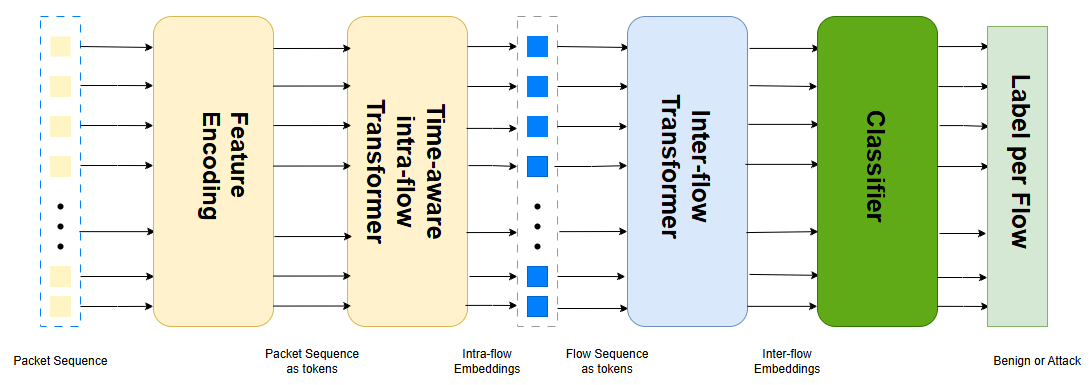
\includegraphics[width=\textwidth]{figures/overall_framework.png}
    \caption{High-level architecture of the hierarchical detector. Stage~1 transforms a packet sequence into an intra-flow representation, and Stage~2 contextualises the resulting flow sequence before classifying the target flow.}
    \label{fig:overall_framework}
\end{figure}

\section{Architectural Overview}
\label{subsec:method_architecture}

Let flow $i$ contain a selected and padded packet-feature matrix
$\mathbf{X}_i\in\mathbb{R}^{L\times d_p}$, a packet inter-arrival tensor
$\mathbf{u}_i\in\mathbb{R}^{L}$, a validity mask
$\mathbf{m}_i\in\{0,1\}^{L}$, a statistical flow vector
$\mathbf{s}_i\in\mathbb{R}^{d_f}$, and a binary target
$y_i\in\{0,1\}$. The principal configuration uses $L=128$. Stage~1 computes

\begin{equation}
    \left(\boldsymbol{\ell}^{(1)}_i,\mathbf{z}^{(1)}_i\right)
    =F_{\theta_1}
    \left(
        \mathbf{X}_i,\mathbf{u}_i,\mathbf{m}_i,\mathbf{s}_i
    \right),
    \label{eq:method_stage1_mapping}
\end{equation}

where $\boldsymbol{\ell}^{(1)}_i\in\mathbb{R}^{2}$ are Stage~1 logits and $\mathbf{z}^{(1)}_i\in\mathbb{R}^{d}$ is the fused representation exported to Stage~2. In the principal model, $d=128$.

After all Stage~1 embeddings have been exported, the flows are stably sorted by start time and flow identifier. For a context relation $r$ and target flow $i$, Stage~2 constructs a bounded causal sequence

\begin{equation}
    \mathbf{Z}^{(r)}_i=
    \left[
        \mathbf{z}^{(1)}_{j_1},\ldots,
        \mathbf{z}^{(1)}_{j_{K_i}},
        \mathbf{z}^{(1)}_i
    \right],
    \qquad j_k<i,\quad K_i\leq W-1,
    \label{eq:method_stage2_input}
\end{equation}

where the current flow is always the last valid token and the principal context window is $W=128$, including the target. Stage~2 predicts

\begin{equation}
    \boldsymbol{\ell}^{(2,r)}_i
    =G_{\theta_2}
    \left(\mathbf{Z}^{(r)}_i,\boldsymbol{\mu}_i\right),
    \label{eq:method_stage2_mapping}
\end{equation}

where $\boldsymbol{\mu}_i$ masks left padding. The final malicious-flow probability is the class-1 softmax output of $\boldsymbol{\ell}^{(2,r)}_i$.

Figure~\ref{fig:method_architecture} shows the information path. Flow labels and Suricata alert fields are targets only and do not enter either encoder.

\begin{figure}[H]
    \centering
    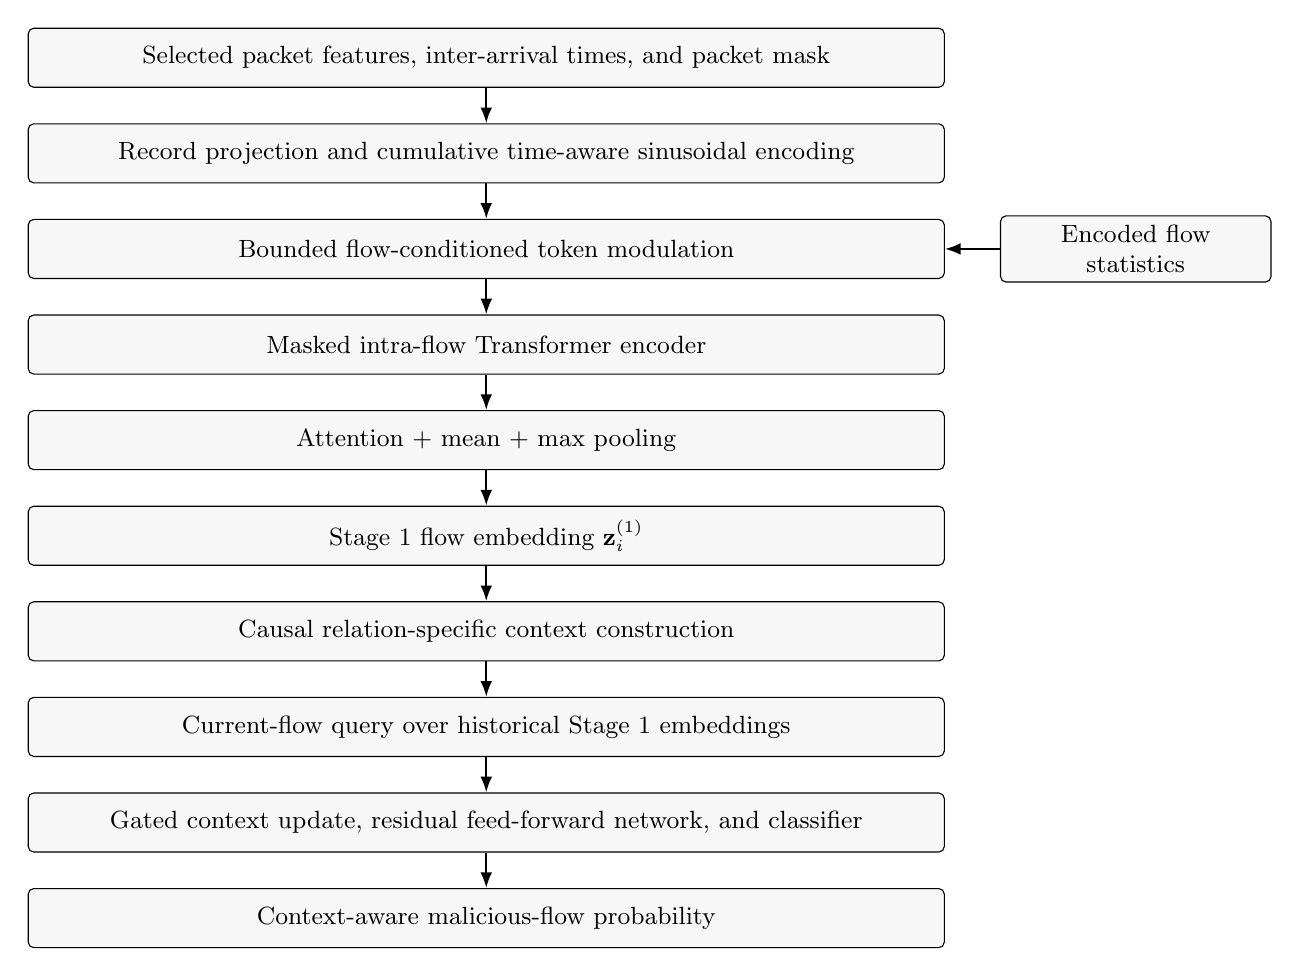
\begin{tikzpicture}[
        node distance=4.5mm,
        block/.style={draw, rectangle, rounded corners=2pt, align=center,
                      text width=11.4cm, minimum height=7.5mm, fill=black!3,
                      font=\small},
        side/.style={draw, rectangle, rounded corners=2pt, align=center,
                     text width=3.2cm, minimum height=8mm, fill=black!3,
                     font=\small},
        arrow/.style={-{Latex[length=2mm]},thick}
    ]
        \node[block] (packet) {Selected packet features, inter-arrival times, and packet mask};
        \node[block, below=of packet] (projection) {Record projection and cumulative time-aware sinusoidal encoding};
        \node[block, below=of projection] (film) {Bounded flow-conditioned token modulation};
        \node[side, right=7mm of film] (flow) {Encoded flow\\statistics};
        \node[block, below=of film] (encoder) {Masked intra-flow Transformer encoder};
        \node[block, below=of encoder] (pool) {Attention + mean + max pooling};
        \node[block, below=of pool] (z) {Stage~1 flow embedding $\mathbf{z}^{(1)}_i$};
        \node[block, below=of z] (context) {Causal relation-specific context construction};
        \node[block, below=of context] (query) {Current-flow query over historical Stage~1 embeddings};
        \node[block, below=of query] (gate) {Gated context update, residual feed-forward network, and classifier};
        \node[block, below=of gate] (output) {Context-aware malicious-flow probability};

        \draw[arrow] (packet) -- (projection);
        \draw[arrow] (projection) -- (film);
        \draw[arrow] (flow) -- (film);
        \draw[arrow] (film) -- (encoder);
        \draw[arrow] (encoder) -- (pool);
        \draw[arrow] (pool) -- (z);
        \draw[arrow] (z) -- (context);
        \draw[arrow] (context) -- (query);
        \draw[arrow] (query) -- (gate);
        \draw[arrow] (gate) -- (output);
    \end{tikzpicture}
    \caption{Detailed architecture of the proposed two-stage detector. The statistical branch conditions Stage~1 packet tokens, while Stage~2 uses the target flow as the query and historical flows as keys and values.}
    \label{fig:method_architecture}
\end{figure}

\section{Stage~1: Intra-Flow Time-Aware Representation}
\label{subsec:method_stage1}

Stage~1 transforms a variable-length packet sequence into one flow embedding. Its principal configuration consists of a record projection, time-aware sinusoidal encoding, flow-conditioned token modulation, a pre-normalised Transformer encoder, hybrid mask-aware pooling, and a two-class prediction head.

\subsection{Packet-Record Projection}
\label{subsubsec:packet_projection}

For packet position $t$, the preprocessed feature vector $\mathbf{x}_{i,t}\in\mathbb{R}^{d_p}$ is projected to the model dimension:

\begin{equation}
    \mathbf{e}_{i,t}
    =\operatorname{LN}
    \left(W_p\mathbf{x}_{i,t}+\mathbf{b}_p\right),
    \qquad
    \mathbf{e}_{i,t}\in\mathbb{R}^{d}.
    \label{eq:record_projection}
\end{equation}

The implementation permits an MLP projection, but the principal configuration uses one linear projection followed by layer normalisation. Categorical packet fields have already been one-hot encoded, numerical fields have been transformed and robustly scaled, and binary fields remain in $\{0,1\}$ as described in Chapter~\ref{sec:dataset_preprocessing}.

\subsection{Cumulative Time-Aware Encoding}
\label{subsubsec:time_aware_encoding}

Conventional sinusoidal positional encoding represents packet order but cannot distinguish two adjacent packets separated by microseconds from two adjacent packets separated by seconds. Stage~1 therefore combines ordinal position with cumulative elapsed time. The preprocessing pipeline stores

\begin{equation}
    u_{i,t}=\log\left(1+\Delta\tau_{i,t}\right),
    \label{eq:stored_log_iat}
\end{equation}

where $\Delta\tau_{i,t}$ is the nonnegative microsecond inter-arrival time from the previous packet in the same bidirectional flow. Inside the model, the interval is reconstructed and masked:

\begin{equation}
    \widehat{\Delta\tau}_{i,t}
    =m_{i,t}\max\left(0,\exp(u_{i,t})-1\right).
    \label{eq:reconstructed_iat}
\end{equation}

The cumulative elapsed time and its smoothed logarithm are

\begin{align}
    c_{i,t} &= \sum_{k=1}^{t}\widehat{\Delta\tau}_{i,k},\\
    p_{i,t} &= \log\left(1+c_{i,t}+\alpha\right),
    \qquad \alpha=10^{-7}.
    \label{eq:cumulative_time_feature}
\end{align}

Let the zero-based packet position be $q_t=t-1$. The combined coordinate is $r_{i,t}=q_t+p_{i,t}$. For channel pair $j$, the time-aware encoding is

\begin{align}
    \operatorname{TE}_{i,t,2j}
    &=\sin\left(
        \frac{r_{i,t}}{10000^{2j/d}}
      \right),\\
    \operatorname{TE}_{i,t,2j+1}
    &=\cos\left(
        \frac{r_{i,t}}{10000^{2j/d}}
      \right).
    \label{eq:time_aware_sinusoid}
\end{align}

Padding positions receive a zero encoding. The encoded packet token is

\begin{equation}
    \widetilde{\mathbf{e}}_{i,t}
    =\operatorname{Dropout}
    \left(
        \mathbf{e}_{i,t}+m_{i,t}\operatorname{TE}_{i,t}
    \right).
    \label{eq:time_encoded_packet}
\end{equation}

This construction follows the time-aware Transformer principle used in GTID \cite{Han2023GTID}, but it is applied here to structured, payload-content-free packet metadata. Position-only and time-only modes are retained as ablations. In the time-only mode, $r_{i,t}=p_{i,t}$; in the position-only mode, $r_{i,t}=q_t$.

\subsection{Flow-Statistics Encoder}
\label{subsubsec:flow_encoder}

The separately preprocessed statistical flow vector $\mathbf{s}_i$ is mapped to the packet-model dimension through a bottleneck encoder:

\begin{equation}
    \mathbf{f}_i
    =\operatorname{LN}_2
    \left(
        W_{f,2}\,
        \operatorname{Dropout}
        \left(
            \operatorname{GELU}
            \left(
                \operatorname{LN}_1(W_{f,1}\mathbf{s}_i+\mathbf{b}_{f,1})
            \right)
        \right)
        +\mathbf{b}_{f,2}
    \right).
    \label{eq:flow_feature_encoder}
\end{equation}

The principal bottleneck dimension is 32 and the output dimension is 128. The bottleneck limits the capacity of the aggregate-feature branch and reduces the risk that high-dimensional flow statistics overwhelm packet-sequence evidence.

\subsection{Bounded Flow-Conditioned Token Modulation}
\label{subsubsec:token_film}

The principal Stage~1 fusion mode is inspired by feature-wise linear modulation (FiLM), in which conditioning information produces feature-specific affine parameters \cite{Perez2018FiLM}. From the flow representation, a small network generates

\begin{equation}
    [\boldsymbol{\gamma}_i;\boldsymbol{\beta}_i]
    =G_f(\mathbf{f}_i),
    \qquad
    \boldsymbol{\gamma}_i,\boldsymbol{\beta}_i\in\mathbb{R}^{d}.
    \label{eq:film_parameters}
\end{equation}

For each packet token, the raw flow-conditioned residual is

\begin{equation}
    \mathbf{r}^{\mathrm{raw}}_{i,t}
    =\eta
    \left(
        \boldsymbol{\gamma}_i\odot\widetilde{\mathbf{e}}_{i,t}
        +\boldsymbol{\beta}_i
    \right),
    \qquad
    \eta=\sigma(a),\qquad a_{0}=-5,
    \label{eq:film_raw_residual}
\end{equation}

where $\odot$ denotes element-wise multiplication. The initial scale is $\sigma(-5)\approx0.0067$. In addition, the residual is constrained relative to the norm of its packet token. With the configured maximum residual ratio $\rho=0.13$,

\begin{align}
    \lambda_{i,t}
    &=\min\left(
        1,
        \frac{\rho\|\widetilde{\mathbf{e}}_{i,t}\|_2}
             {\|\mathbf{r}^{\mathrm{raw}}_{i,t}\|_2+\epsilon}
      \right),\\
    \mathbf{e}^{F}_{i,t}
    &=\widetilde{\mathbf{e}}_{i,t}
      +\lambda_{i,t}\mathbf{r}^{\mathrm{raw}}_{i,t}.
    \label{eq:bounded_token_film}
\end{align}

The final layer producing $\boldsymbol{\gamma}_i$ and $\boldsymbol{\beta}_i$ is initialised to zero. The model therefore begins as the packet-only branch and learns a bounded statistical correction. This is particularly useful when aggregate statistics are predictive but potentially noisy or capture-specific.

The terminology is important. Because the statistical vector is encoded in a separate branch but modulates packet tokens before self-attention, the principal configuration is most precisely described as \emph{separate-branch conditional intermediate fusion}. It is not strict post-pooling late fusion. A post-pooling gated fusion implementation is available as an alternative, but the reported principal Scheme~C configuration uses the bounded token-FiLM mechanism in Equation~\ref{eq:bounded_token_film}.

\subsection{Masked Transformer Encoder}
\label{subsubsec:stage1_transformer}

The conditioned sequence $\mathbf{E}^{F}_i\in\mathbb{R}^{L\times d}$ is processed by a stack of pre-normalised Transformer encoder layers. For layer $\ell$,

\begin{align}
    \mathbf{A}^{\ell}_i
    &=\operatorname{MHA}
      \left(
        \operatorname{LN}(\mathbf{H}^{\ell-1}_i),
        \operatorname{LN}(\mathbf{H}^{\ell-1}_i),
        \operatorname{LN}(\mathbf{H}^{\ell-1}_i);
        \mathbf{m}_i
      \right),\\
    \overline{\mathbf{H}}^{\ell}_i
    &=\mathbf{H}^{\ell-1}_i
      +\operatorname{Dropout}(\mathbf{A}^{\ell}_i),\\
    \mathbf{H}^{\ell}_i
    &=\overline{\mathbf{H}}^{\ell}_i
      +\operatorname{FFN}
       \left(\operatorname{LN}(\overline{\mathbf{H}}^{\ell}_i)\right),
    \label{eq:stage1_transformer_layer}
\end{align}

where $\mathbf{H}^{0}_i=\mathbf{E}^{F}_i$. Each attention head uses scaled dot-product attention

\begin{equation}
    \operatorname{Attn}(Q,K,V)
    =\operatorname{softmax}
      \left(
        \frac{QK^{\top}}{\sqrt{d_h}}+M_i
      \right)V,
    \label{eq:scaled_dot_product_attention}
\end{equation}

where $M_i$ assigns negative infinity to padded key positions. The feed-forward network uses GELU activation. The principal model has two encoder layers, four attention heads, model dimension 128, feed-forward dimension 256, and dropout 0.15.

No causal mask is used inside Stage~1: all retained packets of the completed or truncated flow can attend to one another. Consequently, Stage~1 is a flow-level classifier, not a claim of packet-by-packet early detection. Padding is excluded from attention keys and from the subsequent pooling operation.

\subsection{Hybrid Mask-Aware Pooling}
\label{subsubsec:hybrid_pooling}

The packet states are reduced using three complementary summaries. First, a learned attention score is computed for each valid token:

\begin{align}
    a_{i,t}
    &=\mathbf{w}_{a,2}^{\top}
      \operatorname{GELU}
      \left(W_{a,1}\mathbf{h}_{i,t}+\mathbf{b}_{a,1}\right)+b_{a,2},\\
    \omega_{i,t}
    &=\frac{m_{i,t}\exp(a_{i,t})}
      {\sum_{k=1}^{L}m_{i,k}\exp(a_{i,k})},\\
    \mathbf{z}^{\mathrm{att}}_i
    &=\sum_{t=1}^{L}\omega_{i,t}\mathbf{h}_{i,t}.
    \label{eq:stage1_attention_pooling}
\end{align}

The masked mean and maximum are

\begin{align}
    \mathbf{z}^{\mathrm{mean}}_i
    &=\frac{\sum_{t=1}^{L}m_{i,t}\mathbf{h}_{i,t}}
            {\max(1,\sum_{t=1}^{L}m_{i,t})},\\
    \mathbf{z}^{\mathrm{max}}_i
    &=\max_{t:m_{i,t}=1}\mathbf{h}_{i,t}.
    \label{eq:mean_max_pooling}
\end{align}

The final Stage~1 embedding combines all three:

\begin{equation}
    \mathbf{z}^{(1)}_i
    =\operatorname{Dropout}
      \left(
        \operatorname{GELU}
        \left(
          \operatorname{LN}
          \left(
            W_o
            [\mathbf{z}^{\mathrm{att}}_i;
             \mathbf{z}^{\mathrm{mean}}_i;
             \mathbf{z}^{\mathrm{max}}_i]
            +\mathbf{b}_o
          \right)
        \right)
      \right).
    \label{eq:hybrid_pooling}
\end{equation}

Attention pooling can emphasise a small number of informative packets, mean pooling represents overall behaviour, and max pooling preserves strong local activations. Their concatenation is projected back to dimension $d$ so Stage~2 receives one consistently sized vector per flow.

The Stage~1 class logits are

\begin{equation}
    \boldsymbol{\ell}^{(1)}_i
    =h_1(\mathbf{z}^{(1)}_i),
    \qquad
    \mathbf{p}^{(1)}_i
    =\operatorname{softmax}(\boldsymbol{\ell}^{(1)}_i).
    \label{eq:stage1_classifier}
\end{equation}

The exported embedding is taken before the final two-class layer. It therefore retains information useful for contextual refinement rather than reducing each flow to a single probability.

\subsection{Stage~1 Fusion Variants}
\label{subsubsec:stage1_variants}

The implementation supports the three controlled variants in Table~\ref{tab:stage1_fusion_variants}. They share the same packet features, sequence policy, split, Transformer capacity, training procedure, and classifier unless an experiment explicitly states otherwise.

\begin{table}[H]
    \centering
    \caption{Stage~1 packet/flow integration variants.}
    \label{tab:stage1_fusion_variants}
    \small
    \begin{tabular}{@{}p{1.1cm}p{3.1cm}p{8.9cm}@{}}
        \toprule
        Scheme & Input structure & Integration mechanism \\
        \midrule
        A & Packet + repeated flow statistics & The transformed flow vector is concatenated to every packet before record projection. \\
        B & Packet only & The flow-statistics branch is disabled; this isolates packet order and time-aware encoding. \\
        C & Packet + separate flow branch & The flow vector is encoded once and conditionally modulates packet tokens through bounded token-FiLM. This is the principal proposed Stage~1 configuration. \\
        \bottomrule
    \end{tabular}
\end{table}

\section{Stage~2: Causal Inter-Flow Context Modelling}
\label{subsec:method_stage2}

Stage~2 asks whether a target flow should be interpreted differently when recent related behaviour is available. It operates only on Stage~1 embeddings and context metadata. Raw packet fields, flow statistics, and labels of historical flows are not loaded into the Stage~2 input.

\subsection{Embedding Interface and Chronological Order}
\label{subsubsec:embedding_interface}

Stage~1 exports, for each split,

\begin{equation}
    \left(
      \operatorname{flow\_id}_i,
      y_i,
      \mathbf{z}^{(1)}_i,
      t_i^{0},u_i,v_i,\rho_i
    \right),
    \label{eq:stage1_export_tuple}
\end{equation}

where $t_i^{0}$ is the flow start time, $u_i$ and $v_i$ are source and destination identifiers, and $\rho_i$ is the split. Stage~2 validates unique flow identifiers, concatenates the split files, and stably sorts by $(t_i^{0},\operatorname{flow\_id}_i)$. The embedding rows are reordered with the metadata so their alignment is preserved.

Training embeddings are exported with a deterministic, non-sampled loader. This is essential because the weighted training sampler draws with replacement; using it for export would duplicate some flows and omit others. The weighted sampler is used only for optimisation batches.

\subsection{Relation-Specific Causal Contexts}
\label{subsubsec:context_relations}

The context builder scans the sorted flows once from past to future. Before adding target flow $i$ to any history, it retrieves eligible earlier indices. The four evaluated relations are defined in Table~\ref{tab:context_relations}.

\begin{table}[H]
    \centering
    \caption{Stage~2 context relations.}
    \label{tab:context_relations}
    \small
    \begin{tabular}{@{}p{3.0cm}p{4.0cm}p{7.1cm}@{}}
        \toprule
        Method & Eligibility condition for $j<i$ & Interpretation \\
        \midrule
        \methodfield{time_only} & Always eligible & Most recent flows globally, regardless of endpoint identity. \\
        \methodfield{source_host} & $u_j=u_i$ & Earlier flows initiated by the same source identifier. \\
        \methodfield{destination_host} & $v_j=v_i$ & Earlier flows directed to the same destination identifier. \\
        \methodfield{endpoint} &
        $\{u_j,v_j\}\cap\{u_i,v_i\}\neq\varnothing$ & Earlier flows sharing at least one endpoint in either role. \\
        \bottomrule
    \end{tabular}
\end{table}

For relation $r$, let

\begin{equation}
    \mathcal{A}^{(r)}_i
    =\left\{j<i:R_r(i,j)=1\right\}.
    \label{eq:method_eligible_context}
\end{equation}

After split-policy filtering and deduplication, the most recent $W-1$ indices are retained:

\begin{equation}
    \mathcal{C}^{(r)}_i
    =\operatorname{Recent}_{W-1}
      \left(\mathcal{A}^{(r)}_i\right).
    \label{eq:recent_context}
\end{equation}

The current flow is then appended, producing Equation~\ref{eq:method_stage2_input}. Histories are updated only after this sequence has been built, which prevents self-inclusion and future leakage. The principal context policy is \methodfield{online}: validation flows may use earlier training flows, and test flows may use earlier training, validation, and test flows, but never a future flow. This simulates persistent detector state across chronological deployment. No historical label is exposed.

Here, ``causal'' is defined by the implementation's stable start-time order: every context index precedes the target index. The current Stage~2 export does not enforce $t_j^{\mathrm{end}}\leq t_i^{0}$, so long-lived overlapping flows may appear earlier in that order even if their complete embeddings would not yet be available at the target start time. The experiments therefore establish start-ordered, label-free context rather than a fully timed streaming implementation. A deployment-grade version should construct eligibility from flow-completion or embedding-availability timestamps.

The term \methodfield{time_only} means chronological global recency. It does not mean that continuous inter-flow time gaps are supplied to Stage~2. In the current implementation, Stage~2 encodes relative context age, while explicit microsecond timing is modelled inside Stage~1.

The collate function left-pads short sequences so the target remains at the last valid position:

\begin{equation}
    [\mathrm{PAD},\ldots,\mathrm{PAD},
      \mathbf{z}^{(1)}_{j_1},\ldots,
      \mathbf{z}^{(1)}_{j_{K_i}},
      \mathbf{z}^{(1)}_i].
    \label{eq:left_padded_context}
\end{equation}

The accompanying Boolean mask makes the physical padding positions irrelevant to positional encoding and attention.

\subsection{Context-Age Positional Encoding}
\label{subsubsec:context_age_encoding}

If a target has $K_i$ historical tokens, the target receives age 0, the most recent historical flow receives age 1, and the oldest retained flow receives age $K_i$. Let $a_{i,k}$ denote this age index. Stage~2 adds a conventional sinusoidal encoding

\begin{align}
    \operatorname{PE}_{i,k,2j}
    &=\sin\left(
        \frac{a_{i,k}}{10000^{2j/d}}
      \right),\\
    \operatorname{PE}_{i,k,2j+1}
    &=\cos\left(
        \frac{a_{i,k}}{10000^{2j/d}}
      \right).
    \label{eq:stage2_age_encoding}
\end{align}

Unlike absolute tensor positions, age values are invariant to the amount of left padding. This allows the same target and history order to receive the same encoding in batches with different sequence lengths.

\subsection{Target-Query Gated Multi-Head Attention}
\label{subsubsec:target_query_attention}

The principal Stage~2 model is \methodfield{target_query_gated}. Rather than allowing every historical token to attend to every other historical token, it uses the current flow as one query over the eligible history. Let $\mathbf{c}_i$ be the projected current Stage~1 embedding and let $\widetilde{\mathbf{H}}_i\in\mathbb{R}^{K_i\times d}$ contain age-encoded historical embeddings. For attention head $h$,

\begin{align}
    \mathbf{q}^{h}_i
    &=W_Q^{h}\operatorname{LN}
      \left(\mathbf{c}_i+\operatorname{PE}(0)\right),\\
    \mathbf{K}^{h}_i
    &=\operatorname{LN}(\widetilde{\mathbf{H}}_i)W_K^{h},\\
    \mathbf{V}^{h}_i
    &=\operatorname{LN}(\widetilde{\mathbf{H}}_i)W_V^{h},\\
    \mathbf{h}^{h}_i
    &=\operatorname{softmax}
      \left(
        \frac{\mathbf{q}^{h}_i(\mathbf{K}^{h}_i)^{\top}}
             {\sqrt{d_h}}+M_i
      \right)
      \mathbf{V}^{h}_i.
    \label{eq:target_query_attention}
\end{align}

The head outputs are concatenated and projected to obtain the historical summary $\mathbf{h}_i$. If no eligible historical flow exists, $\mathbf{h}_i=\mathbf{0}$. This explicit fallback prevents a fabricated padding token from contributing context.

The model compares the current representation and context summary through difference and multiplicative interactions:

\begin{align}
    \mathbf{r}_i
    &=[\mathbf{c}_i;\mathbf{h}_i;
       \mathbf{c}_i-\mathbf{h}_i;
       \mathbf{c}_i\odot\mathbf{h}_i],\\
    \mathbf{v}_i
    &=[\mathbf{h}_i;
       \mathbf{c}_i-\mathbf{h}_i;
       \mathbf{c}_i\odot\mathbf{h}_i].
    \label{eq:target_context_interactions}
\end{align}

A dimension-wise gate and context update are then computed:

\begin{align}
    \mathbf{g}_i&=\sigma(G(\mathbf{r}_i)),\\
    \mathbf{d}_i&=U(\mathbf{v}_i),\\
    \mathbf{f}_i&=\operatorname{LN}
      \left(\mathbf{c}_i+\mathbf{g}_i\odot\mathbf{d}_i\right).
    \label{eq:gated_context_update}
\end{align}

When no history exists, both $\mathbf{g}_i$ and $\mathbf{d}_i$ are set to zero, so the model reduces to the current-flow representation. Finally, a residual feed-forward block produces

\begin{align}
    \mathbf{z}^{(2)}_i
    &=\operatorname{LN}
      \left(
        \mathbf{f}_i+\operatorname{FFN}(\mathbf{f}_i)
      \right),\\
    \boldsymbol{\ell}^{(2)}_i
    &=h_2(\mathbf{z}^{(2)}_i).
    \label{eq:stage2_output}
\end{align}

The target-query formulation preserves a strong current-flow path and lets context act as a learned correction. Its attention-score matrix grows linearly with $W$ because it contains one query, whereas full self-attention constructs a $W\times W$ score matrix. This makes a window of 128 flows practical while retaining multi-head retrieval from historical behaviour.
\section{Imbalance-Aware Objective and Stage Interface}
\label{subsec:method_training}

\subsection{Focal Objective and Controlled Sampling}
\label{subsubsec:focal_training}

Both stages use two-class softmax outputs and focal loss. For a sample with label $y_i$ and predicted probability $p_{i,y_i}$,

\begin{equation}
    \mathcal{L}_{\mathrm{focal}}
    =-\frac{1}{B}
      \sum_{i=1}^{B}
      \alpha_{y_i}
      \left(1-p_{i,y_i}\right)^{\gamma}
      \log p_{i,y_i}.
    \label{eq:method_focal_loss}
\end{equation}

Focal loss reduces the influence of easily classified examples and was originally proposed for severe foreground/background imbalance \cite{Lin2017FocalLoss}. The focal exponent, class weights, and label-smoothing settings are experimental choices and are reported in Table~\ref{tab:experimental_training_config}.

Training batches are additionally formed by a controlled weighted sampler. If $n_0$ and $n_1$ are the training counts and the desired expected positive fraction is $q$, each negative and positive example receives

\begin{equation}
    w_0=\frac{1-q}{n_0},
    \qquad
    w_1=\frac{q}{n_1}.
    \label{eq:controlled_sampler}
\end{equation}

The sampler changes expected minority exposure without altering the dataset or the loss definition. Stage-specific sampling targets and loader policies are specified in Chapter~\ref{sec:experimental_methodology}.

\subsection{Sequential Stage Interface}
\label{subsec:sequential_stage_interface}

Stage~1 is trained for flow-level classification and restored from its validation-selected checkpoint. A deterministic, non-sampled loader then exports exactly one $\mathbf{z}^{(1)}_i$ per flow together with the metadata required for causal context construction. Stage~2 treats these embeddings as fixed inputs; its gradients do not update the Stage~1 encoder. This sequential interface ensures that Stage~1 comparisons vary the intra-flow representation, while Stage~2 comparisons reason over one fixed representation.

\providecommand{\ExpPlatform}{Google Colaboratory Pro+}
\providecommand{\ExpComputeBudget}{600 purchased compute units}
\providecommand{\ExpGPU}{NVIDIA L4 (24~GB)}
\providecommand{\ExpCPU}{Google Colab hosted CPU; exact model not retained in the run metadata}
\providecommand{\ExpOS}{Google Colab hosted Linux runtime}
\providecommand{\ExpSoftware}{PyTorch and scikit-learn on CUDA; exact version snapshot not retained}
\providecommand{\ExpSuricata}{Suricata with the custom output module; exact version and revision not retained}

\chapter{Experimental Methodology}
\label{sec:experimental_methodology}

The evaluation protocol fixes the data manifest, preprocessing state, optimisation budget, checkpoint criterion, threshold-selection rule, and random seed within each comparison block. Every model checkpoint is selected by validation PR-AUC, its decision threshold is selected by validation class-1 F1, and final metrics are computed once on the untouched test partition. These controls reduce temporal leakage and test-set feedback, which can otherwise produce optimistic NIDS estimates \cite{SommerPaxson2010,Arp2022DosDonts}.

\section{Evaluation Manifests and Leakage Controls}
\label{subsec:experimental_data_protocol}

The archived experiments contain two chronological evaluation blocks. Stage~1 architecture, encoding, fusion, sequence-length, and selection comparisons use a 35,410-flow test manifest containing 34,003 negative and 1,407 positive flows. The independent Scheme~C reference used in the hierarchical comparison and all Stage~2 experiments use the full 84,380-flow test partition containing 80,860 negative and 3,520 positive flows. The two blocks are not treated as paired evaluations, even when rounded metrics are similar. Effect sizes are reported only within one manifest.

Within each block, models receive the same flow universe, packet and flow tensors, split membership, and training-fitted preprocessing state. Categorical vocabularies, clipping bounds, and scaling parameters are fitted on training data only. Sampler weights use training counts, while configured class weights and sampling targets are selected without test feedback; validation and test data never fit transformations.

Stage~2 uses one frozen Stage~1 checkpoint. Its online context policy permits only embeddings earlier in the stable start-time order: validation examples may retrieve earlier training flows, and test examples may retrieve earlier training, validation, and test flows. Histories are updated only after the current context has been built, and neither future embeddings nor historical labels are retrieved. Every Stage~2 architecture comparison reuses the same embedding files, metadata order, context indices, and masks. These invariants isolate the varied model or context factor from preprocessing and context availability. Section~\ref{subsubsec:context_relations} states the distinction between this start-ordered policy and strict flow-completion-time availability.

\section{Experimental Matrix}
\label{subsec:experimental_matrix}

Table~\ref{tab:experiment_matrix} separates comparisons of the packet encoder from comparisons of the complete hierarchical system.

\begin{table}[H]
    \centering
    \caption{Experimental matrix. Only the factor listed in the final column is changed within each experiment group.}
    \label{tab:experiment_matrix}
    \resizebox{\textwidth}{!}{%
    \begin{tabular}{@{}lllll@{}}
        \toprule
        Group & Stage & Fixed reference & Compared alternatives & Varied factor \\
        \midrule
        S1-E1 & 1 & Stage~1 manifest & Flow MLP; packet sequence models; proposed Stage~1 & Encoder family \\
        S1-E2 & 1 & Scheme B, $L=128$, head & Both, position-only, time-only, no encoding & Temporal/order encoding \\
        S1-E3 & 1 & Both encodings, $L=128$, head & Schemes A, B, C & Flow-statistics integration \\
        S1-E4 & 1 & Scheme B, head & $L=8,16,32,64,128,256$ & Packet budget \\
        S1-E5 & 1 & Scheme B, $L=128$ & Head, head-tail, random & Truncation policy \\
        S2-E1 & 2 & flow manifest; same frozen embeddings & No-context MLP; Transformer; LSTM; GRU; CNN+LSTM; proposed & Context encoder \\
        S2-E2 & 2 & Proposed model, $W=128$ & Time-only, source-host, destination-host, endpoint & Context relation \\
        S2-E3 & 2 & Proposed model, source-host & $W=16,32,64,128,256$ & Context capacity \\
        \bottomrule
    \end{tabular}%
    }
\end{table}

\subsection{Stage~1 Baselines}
\label{subsubsec:stage1_baselines}

The Stage~1 comparison includes the following baselines:

\begin{itemize}[leftmargin=*]
    \item \textbf{Flow-level MLP.} A multilayer perceptron consumes only the aggregated statistical flow vector. It provides the direct reference for testing whether packet-level sequence information adds value beyond conventional flow aggregation.

    \item \textbf{CNN1D.} Parallel one-dimensional convolutions with kernel sizes 3, 5, and 7 capture local packet motifs, followed by global pooling and classification. A second variant concatenates the log inter-arrival feature to each packet record. The design follows the general use of multi-kernel convolution for sequence classification \cite{Kim2014CNN}.

    \item \textbf{LSTM and BiLSTM.} Two-layer recurrent encoders with hidden width 128 and mean pooling provide unidirectional and bidirectional sequence references. The LSTM-with-time variant concatenates the stored log inter-arrival value to each packet vector
    \cite{Hochreiter1997LSTM}.

    \item \textbf{GRU.} A two-layer, width-128 GRU with mean pooling tests whether a lighter gated recurrent encoder is sufficient \cite{Cho2014GRU}.

\end{itemize}

All Stage~1 baselines use the same packet tensors, masks, chronological split, focal objective, sampler, optimizer budget, and model-selection protocol as the proposed model. Model capacity is not forced to be identical; trainable parameter count and runtime are reported with predictive performance so that accuracy--efficiency trade-offs remain visible.

\subsection{Stage~1 Ablations and Sensitivity Tests}
\label{subsubsec:stage1_ablation_protocol}

Four encoding variants isolate the contribution of order and elapsed time: (i) both positional and time-aware encoding, (ii) positional encoding only, (iii) time-aware encoding only, and (iv) neither encoding. These variants keep the packet features and Transformer capacity unchanged. Their comparison is particularly important because concatenating an interval value to a packet vector is not equivalent to using elapsed time as the coordinate of a sinusoidal sequence encoding.

Flow-statistics integration is evaluated through the three schemes defined in Table~\ref{tab:stage1_fusion_variants}. Scheme A repeats flow statistics at every packet position, Scheme B excludes flow statistics, and Scheme C uses a separate flow branch with bounded token-FiLM conditioning. Scheme B is used for packet-encoder and truncation studies because it isolates sequence modelling from flow-statistics fusion. Scheme C is the principal complete Stage~1 model and supplies the embeddings used by Stage~2.

Sequence-length sensitivity is measured with $L\in\{8,16,32,64,128,256\}$ under \texttt{head} selection. Selection-policy sensitivity fixes $L=128$ and compares \texttt{head}, \texttt{head\_tail}, and deterministic \texttt{random} subsampling. All other settings remain unchanged.

\subsection{Stage~2 Baselines and Context Ablations}
\label{subsubsec:stage2_baseline_protocol}

The proposed target-query gated attention model is compared with five controls:

\begin{itemize}[leftmargin=*]
    \item \textbf{No-context MLP} classifies only the current Stage~1 embedding and provides a minimal current-flow-only lower bound. Because it is not capacity matched to the contextual encoders, it is not by itself a causal estimate of the value of history.

    \item \textbf{Vanilla Transformer} applies full self-attention to the same context sequence and classifies its last valid token \cite{Vaswani2017}.

    \item \textbf{LSTM} and \textbf{GRU} replace attention with recurrent context encoders while preserving the Stage~1 inputs, context window, masks, and classifier protocol \cite{Hochreiter1997LSTM,Cho2014GRU}.

    \item \textbf{CNN+LSTM} applies parallel temporal convolutions with kernel sizes 3, 5, and 7 before a two-layer LSTM, combining local pattern extraction with recurrent context modelling \cite{Kim2014CNN,Hochreiter1997LSTM}.
\end{itemize}

For the architecture comparison, contextual baselines receive the same \texttt{source\_host} histories with $W=128$ and the current flow included as the last valid element. With the target included, the maximum historical capacity is $W-1=127$ flows. The no-context model receives the same target embedding but discards all preceding elements.

Context-relation sensitivity fixes the proposed encoder and $W=128$, then changes only the eligibility relation among \texttt{time\_only}, \texttt{source\_host}, \texttt{destination\_host}, and \texttt{endpoint}. Window-size sensitivity fixes \texttt{source\_host} and evaluates $W\in\{16,32,64,128,256\}$. The available run summaries retain predictive metrics and confusion matrices but not per-target context occupancy or context age. The resulting limitation is addressed explicitly in the interpretation of the window experiment.

\section{Training, Model Selection, and Thresholding}
\label{subsec:experimental_training_protocol}

\subsection{Principal Training Configuration}
\label{subsubsec:principal_training_config}

Table~\ref{tab:experimental_training_config} summarises the principal architecture and optimisation settings. AdamW is used in both stages to decouple weight decay from the adaptive gradient update \cite{Loshchilov2019AdamW}. Focal loss reduces the influence of easy examples from the majority class \cite{Lin2017FocalLoss}.

\begin{table}[H]
    \centering
    \caption{Principal optimisation configuration. Values changed in a named ablation are the only exceptions.}
    \label{tab:experimental_training_config}
    \begin{tabular}{@{}p{3.0cm}p{4.6cm}p{5.7cm}@{}}
        \toprule
        Setting & Stage~1 & Stage~2 \\
        \midrule
        Architecture and input & Scheme C; $L=128$; head selection; $d=128$ & Target-query gated attention; source-host; $W=128$; $d=128$ \\
        Batch size & 128 & 128 \\
        Optimizer & AdamW & AdamW \\
        Learning rate & $1\times10^{-4}$ & $3\times10^{-5}$ \\
        Weight decay & $1\times10^{-4}$ & $3\times10^{-4}$ \\
        % Gradient clipping & Global norm 1.0 & Global norm 0.5 \\
        Loss & Focal, $\gamma=1$, $\boldsymbol{\alpha}=[1,1.25]$, no label smoothing & Focal, $\gamma=1$, $\boldsymbol{\alpha}=[1,1.01]$, no label smoothing \\
        Sampler target & 10\% class-1 examples & 5\% class-1 examples \\
        Maximum epochs & 500 & 500 \\
        Early-stopping patience & 25 epochs & 15 epochs \\
        Checkpoint criterion & Validation PR-AUC & Validation PR-AUC \\
        % Random seed & 130 & 130 \\
        \bottomrule
    \end{tabular}
\end{table}

The weighted sampler is used only to construct training mini-batches and draws with replacement. Validation, test, and embedding-export loaders are non-sampled and preserve one row per flow. This distinction prevents the sampler from duplicating flow embeddings or altering the empirical label distribution used for evaluation. Automatic mixed precision is enabled on CUDA. Stage~1 reduces the learning rate when validation PR-AUC plateaus; Stage~2 uses five warm-up epochs followed by cosine annealing.

\subsection{Checkpoint and Decision-Threshold Selection}
\label{subsubsec:experimental_thresholding}

Checkpoint selection and decision-threshold selection are separate and identical for every reported experiment. The checkpoint with the highest validation PR-AUC is restored, after which the class-1 decision threshold is selected using validation predictions only:
\begin{equation}
    \delta^{*}
    =\arg\max_{\delta\in\Delta}
      F_{1,1}^{\mathrm{val}}(\delta).
    \label{eq:validation_threshold_selection}
\end{equation}
For Stage~1, $\Delta$ is the set of thresholds induced by the validation precision--recall curve. Stage~2 evaluates 199 equally spaced values from 0.01 to 0.99. The selected $\delta^{*}$ is frozen before test evaluation and applied without further adjustment. The test partition is not used for checkpoint selection, threshold selection, or hyperparameter tuning.

\section{Evaluation Metrics}
\label{subsec:experimental_metrics}

The implementation uses the metric definitions provided by scikit-learn \cite{Pedregosa2011ScikitLearn}. Label 1 is the alert-derived positive class and label 0 is the negative class. The confusion matrix is always reported in the following orientation:
\begin{equation}
    \mathbf{C}=
    \begin{bmatrix}
        \mathrm{TN} & \mathrm{FP}\\
        \mathrm{FN} & \mathrm{TP}
    \end{bmatrix},
    \label{eq:experimental_confusion_matrix}
\end{equation}
where rows denote true labels and columns denote predicted labels. Stating the orientation prevents an ambiguity that is common when confusion matrices are copied between software packages.

\subsection{Class-Wise and Macro-Averaged Measures}
\label{subsubsec:macro_metrics}

For class $c\in\{0,1\}$, precision, recall, and F1 are
\begin{align}
    P_c &= \frac{\mathrm{TP}_c}
    {\mathrm{TP}_c+\mathrm{FP}_c}, \\
    R_c &= \frac{\mathrm{TP}_c}
    {\mathrm{TP}_c+\mathrm{FN}_c}, \\
    F_{1,c} &= \frac{2P_cR_c}{P_c+R_c}.
    \label{eq:classwise_metrics}
\end{align}
Undefined ratios are assigned zero, matching the implementation's
\texttt{zero\_division=0} setting. The macro-averaged metrics are
\begin{align}
    P_{\mathrm{macro}} &= \frac{P_0+P_1}{2}, \\
    R_{\mathrm{macro}} &= \frac{R_0+R_1}{2}, \\
    F_{1,\mathrm{macro}} &= \frac{F_{1,0}+F_{1,1}}{2}.
    \label{eq:experimental_macro_metrics}
\end{align}

Macro-F1 is the primary F1 reported in this thesis and is denoted simply as ``F1'' in high-level result tables. It weights benign and positive classes equally despite their different frequencies. Macro-precision and macro-recall are the corresponding primary precision and recall measures. Because macro averaging can conceal which error type changed, $P_1$, $R_1$, and $F_{1,1}$ are always reported alongside the macro values.

Accuracy and weighted averages are secondary. On the raw dataset, an always-negative classifier would achieve approximately $96.055\%$ accuracy while obtaining zero positive recall. High accuracy or weighted F1 is therefore not sufficient evidence of an effective intrusion detector.

\subsection{False-Positive Rate and Operational Error Counts}
\label{subsubsec:fpr_metric}

The false-positive rate is
\begin{equation}
    \mathrm{FPR}=\frac{\mathrm{FP}}{\mathrm{FP}+\mathrm{TN}},
    \label{eq:false_positive_rate}
\end{equation}
and the false-negative rate is
\begin{equation}
    \mathrm{FNR}=\frac{\mathrm{FN}}{\mathrm{FN}+\mathrm{TP}}
    =1-R_1.
    \label{eq:false_negative_rate}
\end{equation}
FPR is emphasised because even a small rate can create a large alert volume in a high-throughput network. It is interpreted together with the absolute FP and FN counts for each comparison. For a test partition containing $N_0$ benign flows, the expected number of false alerts at the evaluated operating point is $N_0\times\mathrm{FPR}$.

\subsection{Threshold-Independent Ranking Measures}
\label{subsubsec:ranking_metrics}

ROC-AUC summarises the true-positive rate as the false-positive rate varies over all score thresholds \cite{Fawcett2006ROC}. It measures ranking quality but can remain high when the negative class dominates. PR-AUC focuses on the positive class and is therefore given greater weight for this imbalanced dataset \cite{SaitoRehmsmeier2015}.

The code field named \texttt{pr\_auc} is computed with scikit-learn's \texttt{average\_precision\_score}. It is therefore average precision (AP), not trapezoidal integration of linearly interpolated precision-recall points:
\begin{equation}
    \mathrm{AP}=\sum_{k}(R_k-R_{k-1})P_k,
    \label{eq:average_precision}
\end{equation}
where $P_k$ and $R_k$ are the precision and recall at successive score thresholds. Accordingly, every value reported as PR-AUC in this thesis is average precision. A random ranking has expected AP close to the class-1 prevalence, so the observed value should be interpreted relative to the test partition's positive rate.

\section{Efficiency and Resource Measurement}
\label{subsec:efficiency_protocol}

Experiments were executed in Google Colaboratory Pro+ using a company-funded allocation of 600 compute units and an NVIDIA L4 GPU with 24~GB of memory \cite{GoogleColabFAQ2026,NVIDIAL4ProductBrief}. Compute units govern access to hosted resources rather than representing a fixed quantity of GPU work. Runtime comparisons are made only within one experiment stage because data loading, early stopping, and model-specific execution paths differ between Stage~1 and Stage~2.

Trainable parameter count is obtained directly from model tensors requiring gradients. Stage~1 training time covers the complete fit loop, including validation and checkpointing, and is reported as a descriptive single-run cost because model-specific early stopping and hosted-runtime variation affect total wall time. Stage~2 inference is measured with gradients disabled and the model in evaluation mode. The reported per-flow latency is
\begin{equation}
    t_{\mathrm{flow}}=\frac{T_{\mathrm{test}}}{N_{\mathrm{test}}},
    \qquad
    Q=\frac{N_{\mathrm{test}}}{T_{\mathrm{test}}},
    \label{eq:inference_efficiency}
\end{equation}
where $Q$ is throughput in flows per second. This profile begins after Stage~1 embeddings and context indices have been constructed; it is model-evaluation latency, not end-to-end PCAP-to-alert latency.

\begin{table}[H]
    \centering
    \caption{Execution environment for the reported experiment blocks.}
    \label{tab:experimental_environment}
    \begin{tabular}{@{}p{3.4cm}p{10.0cm}@{}}
        \toprule
        Component & Recorded environment \\
        \midrule
        Hosted platform & \ExpPlatform \\
        Purchased allocation & \ExpComputeBudget \\
        Accelerator & \ExpGPU \\
        Host processor and RAM & \ExpCPU \\
        Operating environment & \ExpOS \\
        Learning software & \ExpSoftware \\
        Traffic extractor & \ExpSuricata \\
        \bottomrule
    \end{tabular}
\end{table}

The exact CPU, software-version snapshot, Suricata version, ruleset snapshot, configuration, custom-module revision, and PCAP checksum were not retained in the available run metadata. This omission limits exact runtime and label-generation replication; these values are reported as unavailable rather than reconstructed retrospectively.
\providecommand{\resultsfigurepath}{figures}
\IfFileExists{figures/stage1_model_comparison.pdf}{}{%
    \renewcommand{\resultsfigurepath}{MScCS/figures}%
}

\chapter{Results and Discussion}
\label{sec:results}

Unless stated otherwise, F1, precision, and recall denote macro averages; class-1 measures are identified explicitly. Interpretation emphasises macro-F1, PR-AUC, class-1 performance, FP, FN, and FPR because accuracy is dominated by the negative class. Effect sizes are reported only between models evaluated on the same test manifest.

\section{Stage~1: Intra-Flow Representation}
\label{subsec:results_stage1}

\subsection{Architecture and Temporal-Encoding Effects}
\label{subsubsec:results_stage1_models}

Figure~\ref{fig:results_stage1_models} compares the Stage~1 model families and encoding ablations on the common flow test set. Table~\ref{tab:results_stage1_errors_efficiency} reports their parameter counts and training times.

\begin{figure}[H]
    \centering
    
\includegraphics[width=\textwidth]{\resultsfigurepath/stage1_model_comparison.pdf}
    \caption{Stage~1 architecture and encoding comparison on the common flow test manifest. The horizontal axis begins at 0.52, and absolute values are printed at the end of each bar.}
    \label{fig:results_stage1_models}
\end{figure}

The position+time Transformer provides the strongest balance in this block, reaching macro-F1 $0.8882$ and PR-AUC $0.8564$. Relative to LSTM+time, the strongest non-Transformer baseline by macro-F1, it gains 2.05 percentage points of macro-F1 and recovers 95 additional positive flows for 10 additional false positives. The difference is therefore visible in both summary metrics and operating-point errors.

The encoding ablation clarifies the contribution of the two coordinates. Position identifies where a packet occurs in the selected sequence, whereas cumulative time distinguishes a rapid burst from the same order spread over a longer interval. Time-only is stronger than position-only, but their combination adds a further 0.64 percentage points of macro-F1 and improves both error types over no encoding. The joint improvement supports ordinal position and elapsed time as complementary descriptions of intra-flow behaviour.

The GRU obtains the lowest FPR ($0.8293\%$), but misses 437 positive flows. The position+time model adds only 14 FP relative to GRU while removing 131 FN. This comparison shows why a low false-alarm rate cannot be interpreted without positive coverage: a conservative detector can suppress alerts by moving errors from FP to FN.

The flow-statistics MLP is the direct test of whether packet dynamics add information beyond aggregation. On the same test composition, its macro-F1 and PR-AUC are $0.7762$ and $0.5604$, versus $0.8882$ and $0.8564$ for the position+time model. FP falls from 853 to 296 and FN from 501 to 306. Aggregate duration, count, and inter-arrival summaries therefore do not recover all of the ordering and local timing evidence preserved by the packet sequence.

Figure~\ref{fig:results_stage1_errors} visualises these operating-point trade-offs; because every model uses the same negative examples, its false-positive bars are directly proportional to FPR.

\begin{figure}[H]
    \centering
    
\includegraphics[width=\textwidth]{\resultsfigurepath/stage1_error_comparison.pdf}
    \caption{Stage~1 false-positive and false-negative counts on the common flow test manifest. FPR is printed beside each FP count.}
    \label{fig:results_stage1_errors}
\end{figure}

Explicit time also reduces both error types for LSTM. The CNN result is mixed: adding time improves its selected operating point but lowers PR-AUC and increases FN. This divergence matters because thresholded F1 describes one operating point, whereas PR-AUC describes score ordering across thresholds. The value of timing information therefore depends on how the encoder represents it; appending an interval feature is not equivalent to using elapsed time as a sequence coordinate.

\begin{table}[H]
    \centering
    \caption{Stage~1 parameter counts and single-run training times measured on an NVIDIA L4 GPU in Google Colab.}
    \label{tab:results_stage1_errors_efficiency}
    \begin{tabular}{@{}lrrr@{}}
        \toprule
        Model & Trainable parameters & Training time (s) & Training time (min) \\
        \midrule
        Position+time Transformer & 344,963 & 4,337.6 & 72.29 \\
        Time-only Transformer & 344,963 & 2,250.5 & 37.51 \\
        Position-only Transformer & 344,963 & 1,994.7 & 33.25 \\
        LSTM+time & 217,346 & 3,556.3 & 59.27 \\
        CNN1D+time & 70,274 & 1,162.4 & 19.37 \\
        GRU & 162,690 & 3,684.4 & 61.41 \\
        LSTM & 216,834 & 3,381.2 & 56.35 \\
        CNN1D & 68,354 & 1,591.0 & 26.52 \\
        BiLSTM & 564,738 & 2,625.7 & 43.76 \\
        No-encoding Transformer & 344,963 & 2,213.9 & 36.90 \\
        \bottomrule
    \end{tabular}
\end{table}

The MLP is omitted from Table~\ref{tab:results_stage1_errors_efficiency} because its parameter count and training time were not archived.

CNN1D+time is the fastest Stage~1 model at 1,162.4 seconds, whereas the position+time Transformer takes 4,337.6 seconds. Although the BiLSTM has more parameters, the proposed encoder is the most expensive recorded run. All models in this block were executed on an NVIDIA L4 GPU, but the values remain descriptive total training costs rather than pure architectural throughput because early stopping, data loading, and hosted-runtime variation affect wall-clock time.

\subsection{Packet and Flow-Statistics Integration}
\label{subsubsec:results_stage1_fusion}

All three schemes in Figure~\ref{fig:results_stage1_fusion} use the same flow test manifest. Scheme A tiles the flow-statistics vector into every packet token, Scheme B uses packet features only, and Scheme C keeps packet and flow representations separate before bounded token-FiLM fusion.

\begin{figure}[H]
    \centering
    
\includegraphics[width=\textwidth]{\resultsfigurepath/stage1_fusion_comparison.pdf}
    \caption{Controlled Stage~1 integration comparison on the common flow manifest. Left: macro metrics and threshold-independent ranking metrics. Right: false-positive and false-negative counts. The score axis is truncated and explicitly labelled.}
    \label{fig:results_stage1_fusion}
\end{figure}

Scheme B outperforms Scheme A by 1.30 percentage points in macro-F1 and 2.38 percentage points in PR-AUC. This result is consistent with the repeated injection of an identical aggregate vector interfering with token-specific evidence, even though Scheme A achieves slightly higher macro-precision. Together with the stronger performance of Scheme C, these results suggest that aggregate flow statistics are more effectively integrated through a separate representation pathway than by being replicated across every packet position.

Scheme C achieves the strongest overall performance, with a macro-F1 of $0.8955$, a PR-AUC of $0.8763$, 267 false positives, and 293 false negatives. Its improvement over the packet-only Scheme B occurs in both error directions, supporting the use of a separate statistical pathway that conditions packet representations rather than replacing packet-level evidence. However, the current comparison evaluates Scheme C as an integrated design and does not isolate the contribution of token-FiLM from the effects of its additional parameters and late-fusion pathway. A parameter-matched concatenation control would therefore be required to attribute the observed gain specifically to token-level modulation.
% Scheme B outperforms Scheme A by 1.30 percentage points of macro-F1 and 2.38 points of PR-AUC. This result is consistent with repeated aggregate vectors interfering with token-specific evidence, even though Scheme A slightly raises macro-precision. Aggregate statistics are most effective in these experiments when represented separately rather than repeated as new observations at every sequence position.

% Scheme C provides the strongest result, with macro-F1 $0.8955$, PR-AUC $0.8763$, 267 FP, and 293 FN. Its improvement over packet-only Scheme B occurs in both error directions, supporting a separate statistical pathway that conditions rather than replaces packet tokens. The comparison supports Scheme C as a complete design, but does not isolate token-FiLM from its additional parameters and fusion path; a parameter-matched concatenation control would be required to attribute the gain specifically to token modulation.

\subsection{Sequence Length and Packet Selection}
\label{subsubsec:results_sequence_length}

Figure~\ref{fig:results_stage1_sensitivity} combines the two Stage~1 sensitivity studies. The line plot examines whether increasing the available packet history produces consistent performance gains, while the grouped bars illustrate the precision--recall trade-off among packet-selection strategies.

\begin{figure}[H]
    \centering
    
\includegraphics[width=\textwidth]
    {\resultsfigurepath/stage1_sensitivity.pdf}
    \caption{Stage~1 sensitivity analysis. Left: maximum packet-sequence length under head selection. Right: packet-selection strategy at $L=128$. Dashed lines identify the selected sequence length. Truncated axes are explicitly labelled.}
    \label{fig:results_stage1_sensitivity}
\end{figure}

Performance is non-monotonic in sequence length. Very short inputs provide weaker ranking performance, suggesting that the earliest few packets do not always contain sufficient discriminative evidence. Increasing the packet budget to $L=128$ yields the strongest observed macro-F1 and the best overall error balance. Extending the budget to 256 packets adds 46 false positives and reduces both macro-F1 and PR-AUC, indicating that a larger packet budget does not necessarily provide additional useful information.

The mechanism underlying this non-monotonic trend cannot be determined from the aggregate sweep alone, because changing the maximum sequence length affects truncation differently for short and long flows. A length-stratified analysis would be required to distinguish genuine dilution by later packets from effects related to flow-length composition or model optimisation. Accordingly, $L=128$ is interpreted as the best observed packet budget for the evaluated capture rather than as a universal packet horizon.

At $L=128$, head and head-tail selection differ by only 0.16 percentage points in macro-F1 and are therefore treated as practically indistinguishable in this single-seed comparison. Random selection reduces the false-positive rate but increases the number of false negatives, corresponding to a more conservative operating point. Head selection is retained as the principal policy because it achieves the strongest observed macro-F1 and attack-class recall, is deterministic, and preserves the earliest contiguous packet prefix without requiring access to the end of the packet sequence. No strong claim is made from the small difference between head and head-tail selection.

\section{Stage~2: Inter-Flow Context}
\label{subsec:results_stage2}

\subsection{Gain over Independent Flow Classification}
\label{subsubsec:results_hierarchical_gain}

Table~\ref{tab:results_hierarchical_gain} gives the principal hierarchical comparison. Both rows use exactly the same flow test manifest. The first row classifies the Scheme C embedding independently, while the second adds causal source-host context to the frozen Stage~1 representation.

\begin{table}[H]
    \centering
    \caption{Independent Stage~1 classification and the complete hierarchical system on the common full-data manifest.}
    \label{tab:results_hierarchical_gain}
    \resizebox{\textwidth}{!}{%
    \begin{tabular}{@{}lrrrrrrrl@{}}
        \toprule
        Model & $P_{\mathrm{macro}}$ & $R_{\mathrm{macro}}$ &
        $F_{1,\mathrm{macro}}$ & $F_{1,1}$ & ROC-AUC & PR-AUC & FPR (\%) \\
        \midrule
        Stage~1 Scheme C & 0.8990 & 0.8919 & 0.8954 & 0.7994 & 0.9890 &
        0.8763 & 0.8249 \\
        Stage~2 source-host & \textbf{0.9328} & \textbf{0.9224} &
        \textbf{0.9275} & \textbf{0.8610} & \textbf{0.9938} &
        \textbf{0.9345} & \textbf{0.5429} \\
        \bottomrule
    \end{tabular}%
    }
\end{table}

The complete Stage~2 system raises macro-F1 by 3.21 percentage points and PR-AUC by 5.82 points over independent Scheme C classification. It removes 228 FP and 205 FN, reducing FPR by approximately 34.2\% relative. Improvement in both error types shows that the complete contextual stage improves the operating balance rather than accuracy alone. This comparison evaluates the hierarchical system as a whole; the architecture controls below distinguish its result from simpler context encoders, while the unmatched no-context capacity limits a purely causal attribution to history.


\subsection{Which Relation Defines Useful Context?}
\label{subsubsec:results_context_relation}

Figure~\ref{fig:results_stage2_context} combines ranking performance with the operational recall--FPR trade-off. The left panel compares macro-F1 and PR-AUC; the right panel places each context relation according to class-1 recall and false-positive rate.

\begin{figure}[H]
    \centering
    
\includegraphics[width=\textwidth]{\resultsfigurepath/stage2_context_analysis.pdf}
    \caption{Stage~2 context-relation ablation at $W=128$. Left: macro-F1 and PR-AUC. Right: class-1 recall versus FPR, where the desirable region is the upper-left corner.}
    \label{fig:results_stage2_context}
\end{figure}

Source-host context gives the strongest balance, with macro-F1 $0.9275$, PR-AUC $0.9345$, and the lowest FPR. A plausible explanation is that repeated outbound behavior from one initiator preserves scanning, retry, or coordinated connection patterns, whereas global recency mixes unrelated traffic and a destination history can mix many benign clients of a popular service. The result is consistent with relational and window-level NIDS findings \cite{Deng2023FlowTopology,MartinReizabal2026FlowWindow}, but the current binary labels cannot verify which attack family produces the advantage.

Endpoint context occupies a high-recall regime: it misses fewer positives but produces more FP. By accepting either endpoint in either role, it increases the chance of retrieving relevant lateral or bidirectional behavior, but also imports a more heterogeneous neighborhood. It may therefore be preferable when missed attacks dominate alert-review cost, whereas source-host is the better default under the thesis's balanced criterion. Time-only context performs worse in ranking and FN, indicating that proximity without an entity relation is too weak a context definition for this capture. 

\subsection{How Much Context Is Useful?}
\label{subsubsec:results_context_window}

\begin{figure}[H]
    \centering
    
\includegraphics[width=\textwidth]
    {\resultsfigurepath/stage2_window_sensitivity.pdf}
    \caption{Source-host context-window sensitivity. Left: macro-F1 and PR-AUC. Right: false-positive and false-negative counts. The dashed line marks the selected window $W=128$.}
    \label{fig:results_stage2_window}
\end{figure}

As shown in Figure~\ref{fig:results_stage2_window}, performance varies non-monotonically with context-window size. A 32-flow window achieves the highest macro-recall, but its 775 false positives indicate that the additional sensitivity comes at a substantial false-alert cost. The 128-flow window instead provides the strongest joint performance, with a macro-F1 of $0.9275$, a PR-AUC of $0.9345$, and the lowest FPR of $0.5429\%$. Extending the window to 256 increases both false-positive and false-negative counts. This pattern is consistent with a finite useful context horizon: insufficient history may omit relevant behavioural structure, whereas increasingly old same-source flows may become less related to the current event.

The non-monotonic trend suggests that context usefulness depends on more than nominal window size alone. However, this interpretation remains a hypothesis rather than a direct measurement of context or attention quality. The current aggregate results do not retain the number and age distribution of valid context items for each target flow, and therefore cannot distinguish the effects of genuinely older evidence, different padding rates, and unequal history coverage. A follow-up analysis should stratify performance by observed context length and elapsed context span. Within the evaluated design, $W=128$ is therefore interpreted as the best empirical operating point for the current capture rather than as a universal optimum.

\subsection{Stage~2 Architecture Comparison}
\label{subsubsec:results_stage2_architecture_comparison}

The architecture comparison holds the Stage~1 embeddings, source-host relation, $W=128$, online causal policy, training objective, optimizer, sampling rule, checkpoint criterion, and validation threshold search fixed. Only the context encoder and its architecture-specific dimensions are changed. Figure~\ref{fig:results_stage2_architectures} compares the six architectures; the second panel reports FP and FN directly so that differences in aggregate F1 scores do not obscure the underlying error trade-off.

\begin{figure}[H]
    \centering
    
\includegraphics[width=\textwidth]
    {\resultsfigurepath/stage2_architecture_comparison.pdf}
    \caption{Stage~2 architecture comparison on the common flow test manifest. Left: macro-F1, class-1 F1, and PR-AUC. Right: threshold-dependent false-positive and false-negative counts. Truncated score axes are labelled.}
    \label{fig:results_stage2_architectures}
\end{figure}

The target-query model provides the strongest overall balance, reaching a macro-F1 of $0.9275$, a class-1 F1 of $0.8610$, and a PR-AUC of $0.9345$. The closest baseline values are $0.9097$ macro-F1 from CNN+LSTM and $0.9141$ PR-AUC from GRU. LSTM attains marginally higher macro-recall, but this isolated advantage does not translate into the strongest threshold-independent ranking performance or the best false-alert balance.

The confusion matrices clarify the practical meaning of this ranking. Relative to the vanilla Transformer, the proposed model removes 177 false positives and 117 false negatives on the same test manifest. LSTM detects 28 additional positive flows, but produces 338 additional false alerts. Thus, the proposed model's macro-F1 improvement cannot be explained by a simple threshold-induced trade-off between false positives and false negatives: it reduces both error types relative to the vanilla attention baseline while substantially improving alert precision over the highest-recall recurrent baseline.

The comparison with vanilla self-attention is consistent with the intended inductive bias. Vanilla self-attention repeatedly updates the entire context sequence before classifying its final valid state. The proposed model instead uses the current flow as a query over preceding related flows and gates the resulting context update. The simultaneous gain in macro-F1 and PR-AUC is consistent with more effective target-centred ranking of minority-class examples. However, the current comparison does not isolate the target-query pattern from all other architectural and parameter-count differences.

The no-context head contains only 514 parameters, compared with 283,522 in the proposed Stage~2 model, and therefore serves as a current-flow-only lower bound rather than a capacity-matched context ablation. Its weaker performance shows that a minimal independent classifier is insufficient, but the full performance gap cannot be attributed exclusively to historical context. A stronger controlled ablation would retain the target-query architecture and comparable parameter count while masking all historical context items.

\subsection{Efficiency and Operational Trade-Offs}
\label{subsec:results_statistical_efficiency}

Figure~\ref{fig:results_stage2_efficiency} relates model parameter count to measured model-evaluation latency, with macro-F1 annotated for each architecture. A logarithmic parameter axis is used because model sizes range from 514 to more than 1.2 million parameters.

\begin{figure}[H]
    \centering
    
\includegraphics[width=0.88\textwidth]
    {\resultsfigurepath/stage2_efficiency.pdf}
    \caption{Stage~2 performance--efficiency trade-off. Latency covers model evaluation after Stage~1 embeddings and context indices have been built; it is not end-to-end PCAP-to-alert latency.}
    \label{fig:results_stage2_efficiency}
\end{figure}

All Stage~2 profiles in Figure~\ref{fig:results_stage2_efficiency} were collected on an NVIDIA L4 accelerator. The proposed model contains 283,522 parameters and requires 0.1965~ms per flow for the measured model-evaluation path, equivalent to an average model-level processing rate of approximately 5,089 flows per second under the measured setting. Its latency is effectively identical to the vanilla Transformer's 0.1967~ms; the 0.0002~ms difference is below the resolution needed for a meaningful speed claim. The relevant result is therefore latency parity while achieving a stronger error balance, rather than an acceleration over vanilla attention.

Relative to GRU, LSTM, and CNN+LSTM, the proposed model uses $59.0\%$, $69.3\%$, and $76.7\%$ fewer parameters, respectively. Its measured latency is lower by $42.2\%$, $43.3\%$, and $45.2\%$. Unlike the negligible difference from vanilla attention, these margins indicate a meaningful compactness and model-level latency advantage over the recurrent alternatives. They should not, however, be interpreted as end-to-end deployment throughput. The measurement excludes context-index construction, Stage~1 inference, Suricata extraction, and PCAP processing. In addition, a single aggregate timing does not quantify warm-up effects, run-to-run variance, batching sensitivity, or tail latency.

\section{Cross-Stage Discussion}
\label{subsec:results_cross_stage_discussion}

The two stages address different information losses. Stage~1 recovers packet order and elapsed time that disappear when a flow is reduced to aggregate statistics, whereas Stage~2 recovers behavioural evidence that is unavailable when flows are classified independently. The ablations support both parts of this decomposition. Position and time are complementary within a flow, while causal, start-time-ordered source-host history improves the complete detector after the Stage~1 representation has been fixed. This hierarchical result extends the motivation of packet-aware systems such as GTID and modular flow encoders such as FlowTransformer by evaluating an additional, explicit cross-flow reasoning layer \cite{Han2023GTID,Manocchio2024FlowTransformer}.

For RQ1, the evidence supports time-aware packet-sequence modelling over the flow-statistics MLP on the shared Stage~1 manifest, and the fusion study suggests that aggregate statistics remain useful when they condition rather than replace the packet representation. The non-monotonic sequence-length response is equally important: the observed gain depends on selecting and encoding informative packets rather than increasing the token budget without limit. For RQ2, the aligned flow comparison shows that Stage~2 reduces both false-positive and false-negative counts relative to independent Scheme~C predictions. The relation and window ablations further indicate that context must be selective; merely exposing a model to more neighbouring flows is insufficient.

The combined findings are consistent with broader temporal and relational NIDS work, including sequential traffic modelling and graph-based flow analysis \cite{LiuPatras2022NetSentry,Deng2023FlowTopology,Xu2024SSLGNN}. However, the present experiments do not establish that a single fixed source-host relation captures every attack mechanism, and the binary labels do not reveal which attack families benefit most from contextual modelling. An aligned error-transition analysis would further strengthen the cross-stage interpretation by identifying which Stage~1 false positives and false negatives are corrected by Stage~2 and relating those corrections to context size, context age, and relation type.

Overall, the two stages indicate that intra-flow temporal structure and selective inter-flow relations address distinct information losses that arise when network flows are represented only through aggregate statistics and classified independently.
% \section{Cross-Stage Discussion}
% \label{subsec:results_cross_stage_discussion}

% The two stages address different information losses. Stage~1 recovers packet order and elapsed time that disappear when a flow is reduced to aggregate statistics; Stage~2 recovers behavioural evidence that is unavailable when flows are classified independently. The ablations support both parts of this decomposition. Position and time are complementary within a flow, while start-ordered source-host history improves the complete detector after the Stage~1 representation has been fixed. This hierarchical result extends the motivation of packet-aware systems such as GTID and modular flow encoders such as FlowTransformer by testing an additional, explicit cross-flow reasoning layer \cite{Han2023GTID,Manocchio2024FlowTransformer}.

% For RQ1, the evidence supports time-aware packet-sequence modelling over the flow-statistics MLP on the shared Stage~1 manifest, and the fusion study suggests that aggregate statistics remain useful when they condition rather than replace the packet representation. The non-monotonic sequence-length response is equally important: the gain follows from selecting and encoding informative packets, not from increasing the token budget without limit. For RQ2, the aligned flow comparison shows that Stage~2 lowers both false-positive and false-negative counts relative to independent Scheme~C predictions. The relation and window ablations further indicate that context must be selective; merely exposing a model to more neighbouring flows is insufficient.

% The combined findings are consistent with broader temporal and relational NIDS work, including sequential traffic modelling and graph-based flow analysis \cite{LiuPatras2022NetSentry,Deng2023FlowTopology,Xu2024SSLGNN}. Together, the stages show that intra-flow timing and selective inter-flow relations address distinct information losses in independently aggregated flow classification.


\chapter{Conclusion and Future Work}
\label{sec:conclusion_future_work}

\section{Conclusions}
\label{subsec:conclusion_rq_answers}

\paragraph{RQ1: intra-flow representation.}
The results show that modelling packets as an ordered, time-aware sequence provides a stronger intra-flow representation than relying only on aggregate flow statistics. Positional order and elapsed time provide complementary information, while integrating flow statistics through a separate conditioning and fusion pathway further improves the complete Stage~1 representation. The sequence-length experiments also show that performance does not increase monotonically with the number of observed packets.

\paragraph{RQ2: cross-flow context.}
The results further show that selective historical context improves classification beyond independent flow prediction. Among the tested relations, source-host context provides the strongest overall balance, while endpoint context shifts the operating point towards higher recall at the cost of more false positives. The proposed target-query model achieves the strongest overall performance among the evaluated Stage~2 architectures.

Together, these findings answer the central research question by showing that intra-flow temporal structure and selective inter-flow context provide complementary information at different levels of the detection hierarchy. The main contribution is therefore the evaluated two-stage decomposition and the evidence that these information sources can be combined to improve flow-level intrusion detection, rather than the use of a Transformer architecture in isolation.

\section{Limitations and Scope}
\label{subsec:conclusion_limitations}

The conclusions are bounded by one organisational capture and alert-derived binary labels. Label~0 denotes the absence of a configured Suricata alert rather than independently verified benign traffic, and binary targets do not reveal which attack families benefit from a particular context relation. The experiments use a fixed seed and do not estimate training variability; small differences between nearby configurations are therefore descriptive, and no statistical-significance claim is made \cite{ReimersGurevych2017,Bouthillier2021Variance}. Cross-network, cross-time, and cross-ruleset transfer remain untested.

Stage~2 is causal under stable flow-start order, but does not require a historical flow embedding to have become available before the target flow starts. The no-context baseline is also not capacity matched to the proposed contextual model. Sequential training with frozen Stage~1 embeddings prioritises experimental separation over end-to-end optimisation. Finally, reported Stage~2 latency begins after embeddings and context indices are available and therefore excludes PCAP processing, Suricata extraction, Stage~1 inference, production memory, tail latency, and concept drift.

\section{Future Work}
\label{subsec:conclusion_future_work}

The principal methodological extensions are resource-efficient pre-training for Stage~1 and attack-adaptive, relation-aware context modelling for Stage~2. Both require stronger statistical and external validation.

\subsection{Resource-Efficient Self-Supervised Pre-Training}
\label{subsubsec:future_pretraining}

The current Stage~1 encoder is trained from supervised binary labels. This is practical for the available experiment, but it limits representation learning to the information exposed by a relatively small set of alert-derived labels. Resource constraints prevented large-scale pre-training in the present study. A primary direction for future work is therefore to pre-train the Stage~1 encoder on a larger collection of unlabeled packet and flow records before fine-tuning it for intrusion detection. Self-supervised traffic pre-training has the potential to learn reusable structural representations without requiring payload inspection or a label for every flow
\cite{2024MAETraffic,Dong2025EncryptedPretrain}.

Several pre-training objectives are compatible with the current feature space. Masked packet-feature modelling could reconstruct selected header, direction, length, and timing attributes. Predictive objectives could estimate the next packet's direction, discretised length, or log inter-arrival time. Temporal-order verification could distinguish correctly ordered packet sequences from perturbed sequences, while contrastive learning could align two valid subsequences or augmented views of the same flow. Identity-like fields such as raw IP addresses and ports should be removed or carefully randomised during these tasks so that the encoder learns traffic behaviour rather than memorising hosts.

Pre-training does not eliminate computational cost; it moves additional cost to an offline representation-learning phase. For this reason, future experiments should investigate mixed-precision training, gradient accumulation, moderate sequence lengths, parameter sharing, and progressive training on increasingly large traffic samples. Downstream evaluation should compare random initialisation, frozen-encoder linear probing, partial fine-tuning, and full fine-tuning under equal labelled-data budgets. The key question is not only whether pre-training raises in-domain macro-F1, but whether it improves label efficiency, rare-attack detection, convergence speed, and transfer to later or external captures.

\subsection{Attack-Adaptive Relation-Aware Context Modelling}
\label{subsubsec:future_relation_aware_context}

The Stage~2 experiments show that context quality depends on how related flows are defined. Source-host context provides the best aggregate error balance, whereas endpoint context produces higher attack recall with more false positives. This suggests that no single relation is necessarily optimal for all attack mechanisms. Scanning may be represented by one source contacting many destinations, distributed denial-of-service activity by many sources contacting one destination, brute-force behaviour by repeated service interactions, and lateral movement by a chain of temporally connected endpoints. Future Stage~2 models should therefore select context according to the target flow and the behaviour being modelled rather than relying on one globally fixed relation.

A relation-aware Transformer could construct one causal context pool containing source-host, destination-host, endpoint, protocol, service, subnet, and time-neighbour relations. Each context item would receive a learned relation embedding or relation-specific attention bias. Alternatively, separate key--value projections could be learned for each relation and combined through a target-conditioned gate. In either design, only embeddings available at the target's decision time should remain eligible. Enforcing this with flow-end or embedding-availability timestamps would strengthen the current start-ordered constraint. The context horizon could also be adaptive: a model could choose between a time-duration window and a flow-count window according to recent traffic density.

Evaluation of this extension requires attack-family labels or a defensible behavioural grouping in addition to the current binary target. Results should report per-family relation weights, recall, FPR, and confusion patterns to test whether different attacks actually use different contexts. Comparisons must include the current single-relation model, a relation-agnostic Transformer, and parameter-matched multi-relation controls. Host identifiers should be masked in cross-time and cross-site tests so that relation-aware attention cannot obtain its apparent gain by memorising machines associated with historical alerts. Relation weights may help analysis, but they should not be treated as causal explanations without relation ablation and counterfactual context removal.

% \subsection{Statistical and External Validation}
% \label{subsubsec:future_validation}

% The principal Stage~1 and Stage~2 comparisons should be repeated with at least three to five random seeds. Each run should archive the configuration, validation-selected threshold, checkpoint, test labels, probabilities, and predictions. These aligned outputs would support confidence intervals, paired bootstrap comparisons, McNemar tests, calibration analysis, genuine precision--recall curves, and error-transition analysis between the two stages. The models should then be evaluated on chronologically later captures, unseen hosts, public benchmarks, and, where governance permits, other organisational networks. This would distinguish in-domain performance from temporal, cross-site, and attack-family transfer.

\subsection{Streaming Deployment, Efficiency, and Robustness}
\label{subsubsec:future_streaming_deployment}

The causal formulation is compatible with online inference, but a streaming implementation remains to be validated. Future work should maintain bounded per-relation buffers, evict expired flows, handle out-of-order records, and define behaviour under packet loss, timestamp noise, feature missingness, NAT, and highly shared servers. Evaluation should cover the full path from PCAP processing and Suricata extraction through both model stages and alert generation. In addition to predictive performance, it should report throughput, peak memory, and median, 95th-percentile, and 99th-percentile latency under realistic load.

\bibliographystyle{unsrt}
\bibliography{sources}


\end{document}
